\documentclass[a4paper,11pt,twoside,openright]{WCarticle}


\renewcommand{\gHeader}{Bachelor Thesis}
\renewcommand{\gTitle}{Localized Conformance and Performance Analysis based on Event Data: Diagnosing Individual Places}
\renewcommand{\gAuthor}{Daniel Tacke genannt Unterberg}
\renewcommand{\gSupervisor}{Prof. Wil M.P. van der Aalst\\
Prof. Martin Grohe}
\renewcommand{\gInstitution}{PADS RWTH University}

\begin{document}
%%% Title page
\pagenumbering{roman}

\tpage
\pagestyle{plain}
%%% TOC





%\begin{abstract}
\chapter*{Abstract} \addcontentsline{toc}{chapter}{Abstract}
Nowadays, event data is being generated by many different sources. From process aware information systems (PAIS) to social media and medical devices.
Answering questions about conformance and performance of the processes behind the logged data is the goal of all process mining activities.

To fully uncover complex patterns and problems in the process, several perspectives on the data need to be combined.
Additionally, since some problems may only occur at certain times or stages in the process, the analysis needs to be fine grained.
Most state-of-the-art approaches average over the entire process duration which obscures many weak or rare patterns.

To consider the different perspectives in higher detail, we propose an approach to localize conformance and performance to individual places in a model and time intervals of the process duration.
%\end{abstract}

\tableofcontents


%\setcounter{page}{1}
\cleardoublepage
%%% Begin document
\pagestyle{fancy}
\chapter{Introduction} \label{chap:intro}\pagenumbering{arabic}
%\documentclass[../main.tex]{subfiles}
%\begin{document}
\emph{Process mining} is a relatively new discipline that bridges the gap of data mining and business process management. The objective of process mining is to support the analysis of business processes, provide valuable insights in processes and further improve the business execution based on the business execution data which is recorded in event logs. According to \cite{van2011process}, process mining techniques are divided into three categories: \emph{process discovery}, \emph{conformance checking}, \emph{and process enhancement}. \emph{Process discovery} techniques derive visual models from event logs of the information system, aiming at a better understanding of real business processes. \emph{Conformance checking} analyzes the deviations between a referenced process model and observed behaviors driven from its execution. \emph{Process enhancement} adapts and improves existing process models by extending the model with additional data perspectives or repairing the existing model to accurately reflect observed behaviors. 

Most of the organizations have predefined process execution rules which are captured in a process model. However, in real life, business processes often encounter exceptional situations where it is necessary to execute process differing from the reference model. To reflect reality, the organizations need to adjust the existing process model. Basically, one can apply process discovery techniques again to obtain a new model only based on the event log. However, there is a need that the improved model should be as similar as possible to the original model while replaying the current process execution\cite{fahland2012repairing}. In this situation, the rediscovery method tends to fail due to the ignorance of the impact from the existing model. To meet this need, \emph{model repair} techniques are proposed in \cite{fahland2012repairing}.

\emph{Model repair} belongs to process enhancement\cite{fahland2012repairing}. It analyzes the workflow deviations between an event log and a process model, and fix the deviations mainly by adding subprocesses on the model. As known, organizations are goal-oriented and aims to have high performance according to a set of Key Performance Indicator(KPI)s,e.g. average conversion time for the sales, payment error rate for the finance.  However, little research in process mining is conducted on the basis of business performance\cite{ghasemi2019event}.  The authors of \cite{ghasemi2019event} point out several contributions like \cite{dees2017enhancing} to consider business performance into process mining. The work in \cite{dees2017enhancing} divides deviations of model and the event log into positive and negative according to certain KPIs. Then it applies repair techniques in \cite{fahland2015model} only with positive deviations, to avoid introducing negative instances into the repaired model. 

However, the current repair methods have some limits. Model repair techniques fix the model by adding subprocesses. They guarantee that the repaired model replays well the event log but overgeneralizes the model, such that it allows more behaviors than expected. Furthermore, it increases the model complexity.  Even the performance is considered in \cite{dees2017enhancing}, but only deviations in positive is used to add subprocesses, the negative information is ignored, which disables the possibility to block negative behaviors from model. 

In the following part, motivating examples are given to describe those limits of the current repair techniques in several situations. Then we propose research questions to overcome those limits and define our research scope. At the end, we give the outline for the whole thesis.
%% Motivation 
\section{Motivating Examples}
\begin{wrapfigure}{r}{0.3\textwidth}
	\centering
	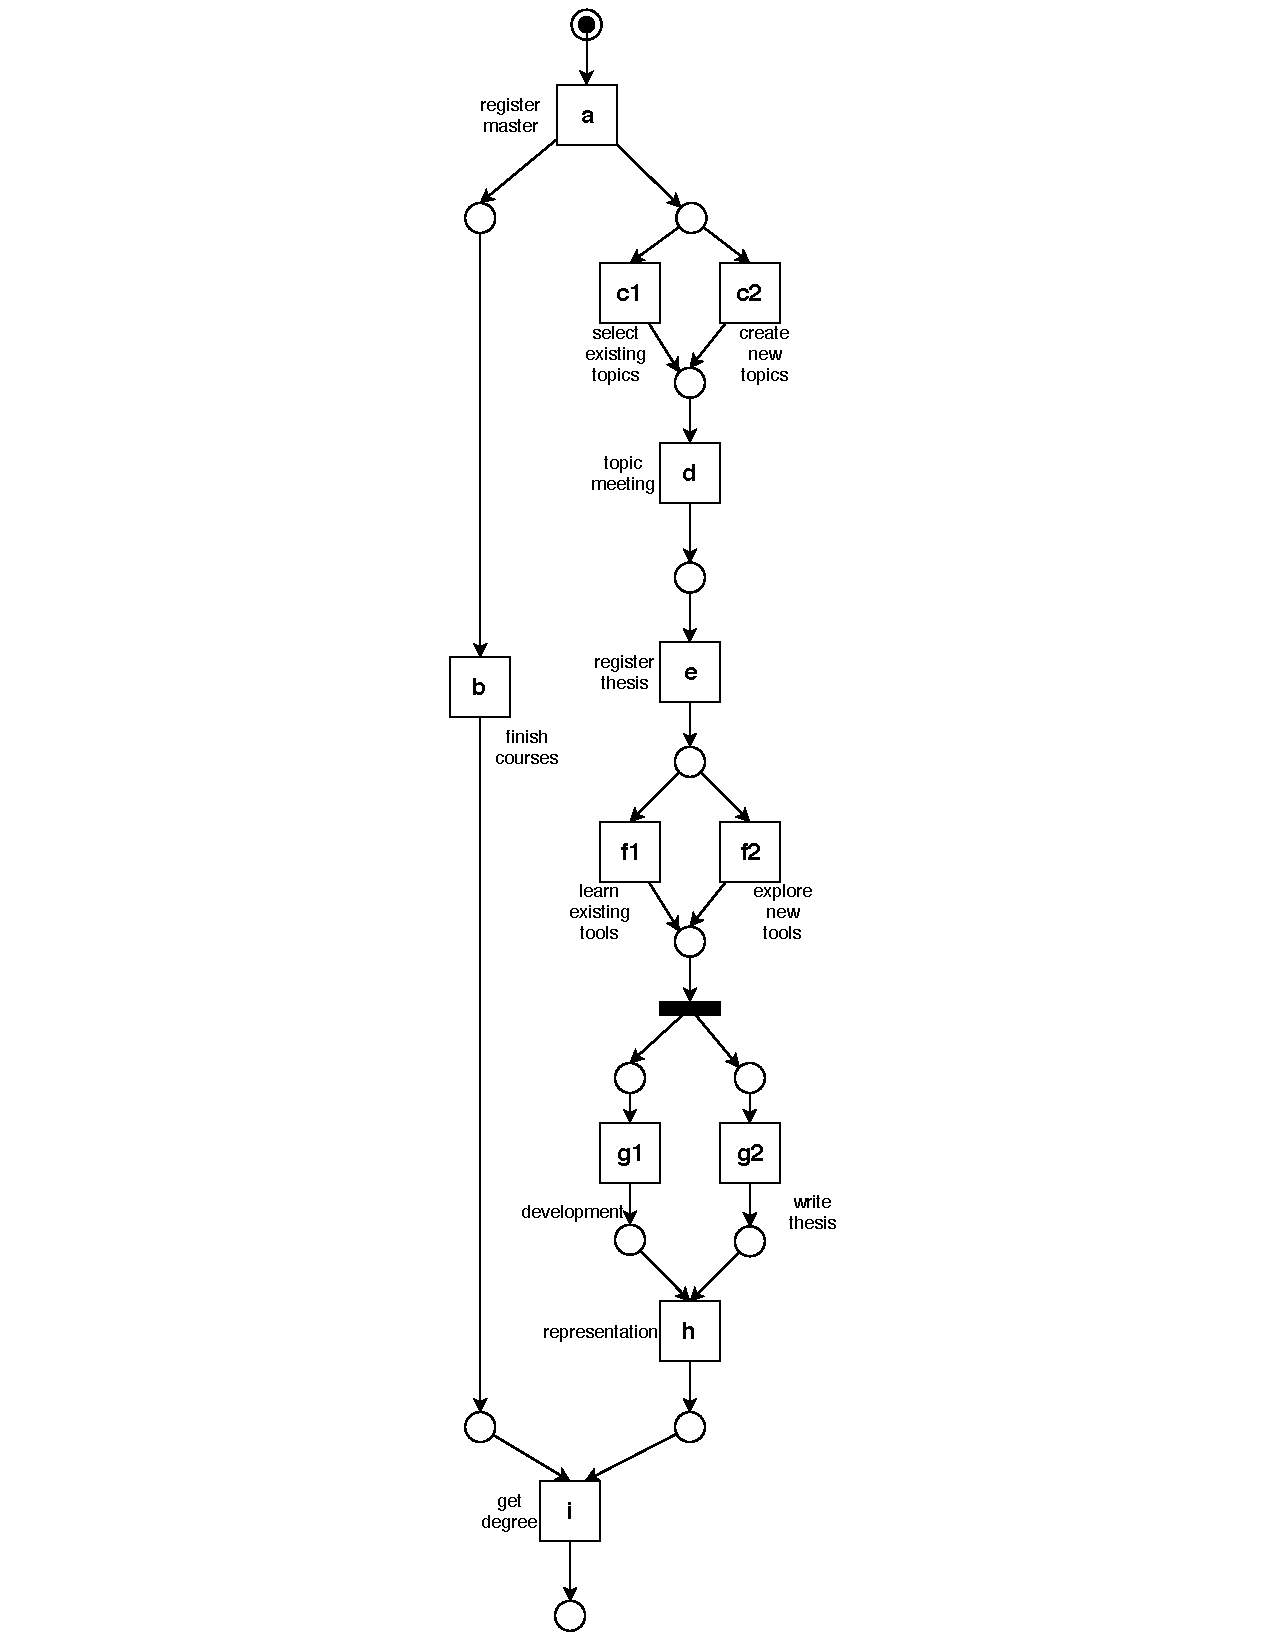
\includegraphics[clip, trim=7cm 0cm 7cm 0cm, width=0.4\textwidth, height=0.7\textheight]{figures/introduction/Master-original-model.pdf}
	\caption{original master study process $M_0$}
	\label{fig:model_M0}
\end{wrapfigure}
% In this section, we use thesis registration example to display the shortcomings of existing techniques and then introduces our methods, but we need to answer them later..
This section describes some situations where current repair techniques tend to fail. For the sake of understanding, examples are extracted from the common master study procedure to illustrate those situations.

The main activities for the master study include \emph{register master}, \emph{finish courses} and \emph{write a master thesis}. Here, we simplify the \emph{finish courses} and only extend the activity \emph{write a master thesis} into a set of sub activities. Those activities are shown in the Petri net model $M_0$ of Figure \ref{fig:model_M0}. The activities are modeled by the corresponding \textbf{\emph{transitions}} which is represented by a square. Transitions are connected through a circle called \textbf{\emph{place}}. Transitions and places build the static structure of Petri net and describe the transition relations. \textbf{\emph{Tokens}} in the black dot are put in the initial places and represent the dynamic state of the model. 

$M_0$ is currently in an initial state where only one token is at the start place to enable the transition \emph{register master}. After firing \emph{register master}, the token at the initial place is consumed while two new token are generated in the output places of \emph{register master}. In this way, activity \emph{finish courses}  can be executed concurrently the other branch except for the \emph{get degree}. When multiple activities have the same input place, all of them are enabled but only one of them can be fired and executed, namely, they are exclusive to each other. As shown in the figure,  \emph{select existing topics}  and \emph{create new topics} are exclusive, and only one of them can be triggered. When a transition has multiple input places, it can be triggered with condition that all input places hold at least a token. \emph{Get degree} is enabled only after \emph{finish courses} and \emph{representation} done. 


% here we are going to talk about the situations where the current repair method can not handle well.
%talk about the execution trace definition. 
% but how to combine them into one example?? I don't think it clearly here. But I need to show it later.
Along the tokens flowing through the model, activities get fired and generate a sequence according to their execution order. One execution sequence is called a trace. A set of traces depicts the model behavior and is recorded into a data file called event log. In real life, activities might be executed with deviation to the process model. A trace which has no deviation to the model is fitting. Otherwise, it's a unfitting trace. With accumulation of deviations, process model needs amending to reflect reality.  In the following part, different several situations are introduced to demonstrate the shortcomings of current techniques to repair a model. 
\subsection{Situation 1: \small{Repairing Model with Unfitting Traces}} % add preparation to this model
In some universities, before registering a master thesis, the activities \emph{write proposal} and \emph{check course requirement} with exclusive choice relation might be necessary in the master study procedure. The real process are recorded in the event log $L_1$. Traces with either of those activities are considered as positive. For convenience, alphabet characters are used to represent the corresponding activities and annotated in the model. \textbf{x1, x2} represent the activities \emph{write proposal} and \emph{check course requirement}.
\emph{Event Log $L_1$ -- }
		\begin{align*}
		Positive:\{ & { <a,b, c1,d,e,\textbf{x1},f1,g1,g2,h,i>}^{50}, \\   &{<a,b, c2,d,e,\textbf{x2},f2,g2,g1,h,i>}^{50} \}
		% Negative: \{ & {<a,c1,d,\quad f,g1,g2,h,i>}^{50} \}
		\end{align*}
\begin{figure}[htp]
	\centering
	\begin{subfigure}[b]{0.5\textwidth}
		\centering
		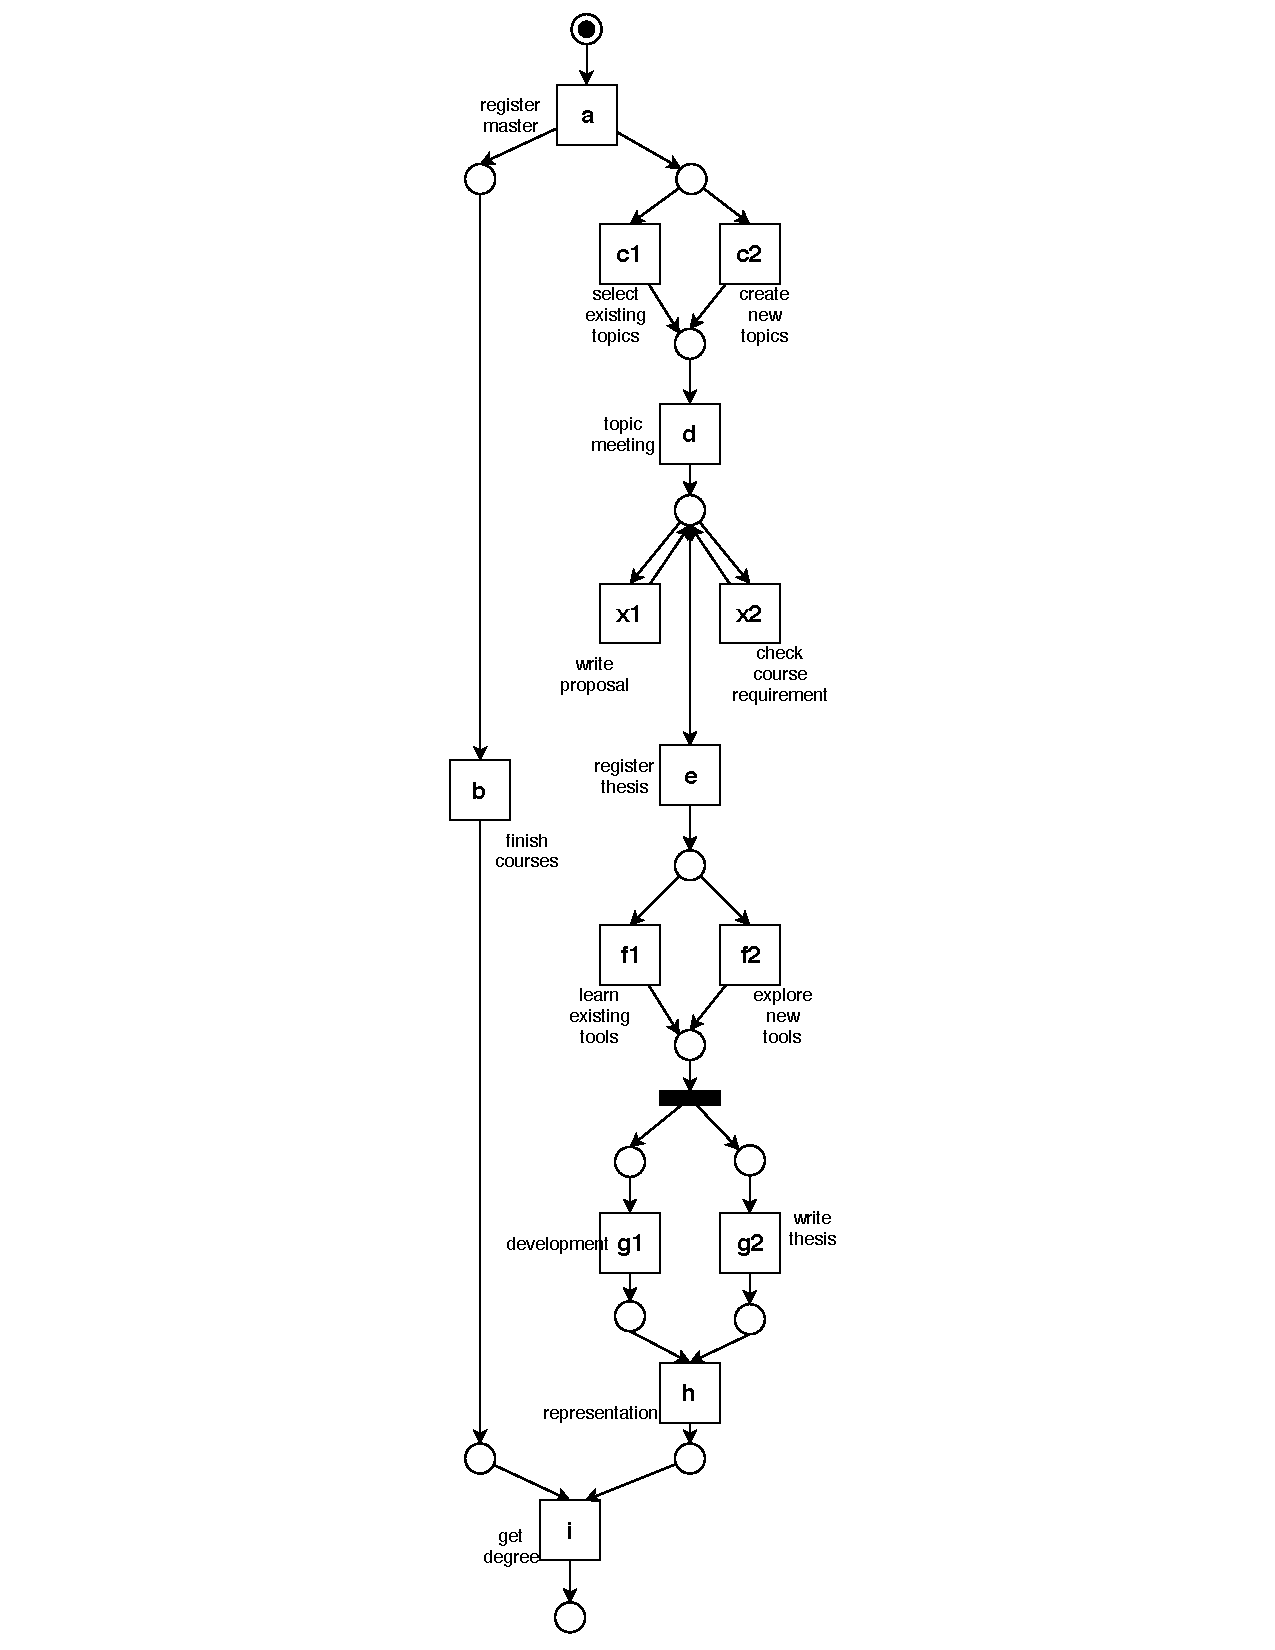
\includegraphics[clip, trim=7cm 0cm 7cm 0cm, width=0.5\linewidth, height=0.7\textheight]{figures/introduction/Master-add-events-loop.pdf}
		\caption{repaired model $M_{1.1}$ with additional activities }
		\label{fig:model_b1}
	\end{subfigure}%
	\begin{subfigure}[b]{0.5\textwidth}
		\centering
		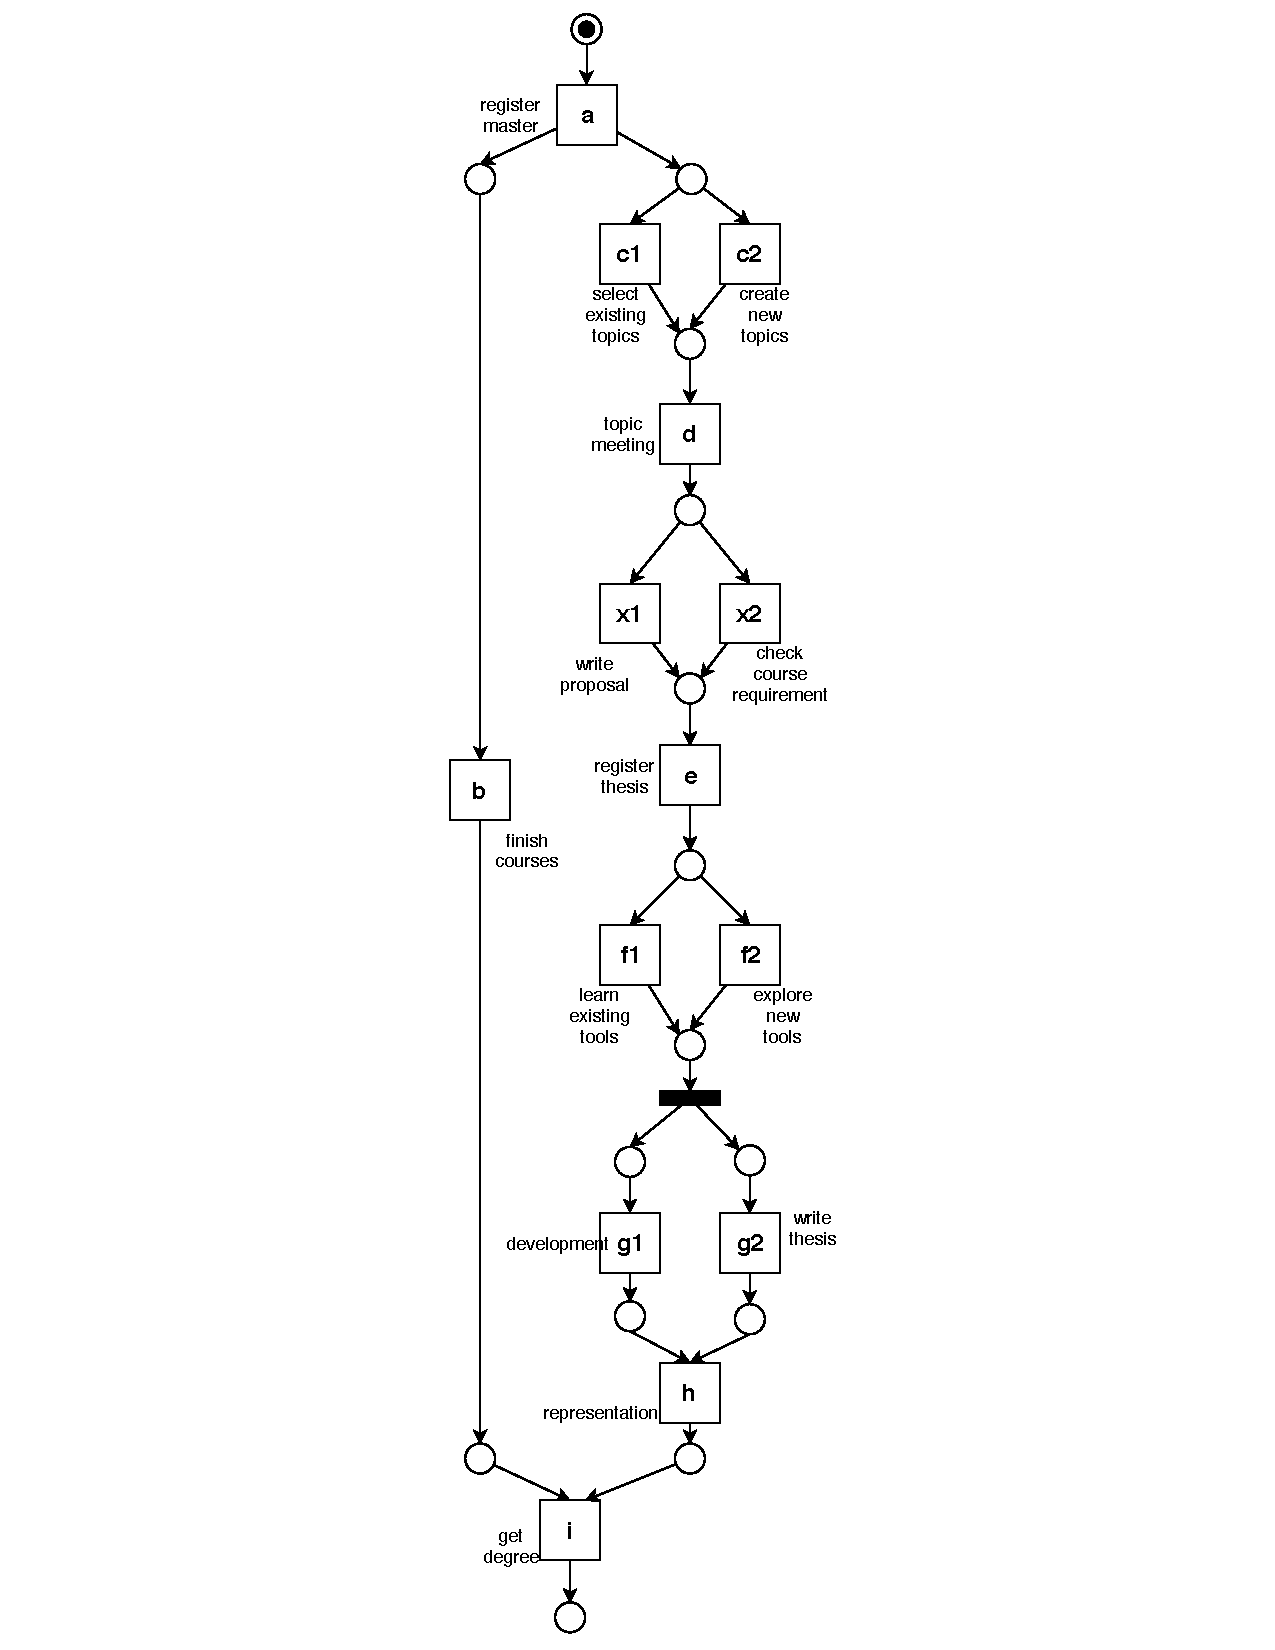
\includegraphics[clip, trim=7cm 0cm 7cm 0cm, width=0.5\linewidth, height=0.7\textheight]{figures/introduction/Master-add-events.pdf}
		\caption{expected model $M_{1.2}$ with additional activities}
		\label{fig:model_b2}
	\end{subfigure}
	\caption{example for situation 1 where $M_{1.1}$ is repaired by adding subprocess in the form of loops, which results in lower precision compared with the expected model $M_{1.2}$.}
	\label{fig:model_change_1}
\end{figure}

Because the existing repair techniques \cite{fahland2015model} don't consider the performance of traces in event log, all instances with positive labels are used to repair the model. Firstly, the deviations of the existing model M0 and the event log $L_1$ are computed. After computation of deviations, each deviation has the same start and end place and two deviations appear at the same position in the model. When repairing this model, each subprocess has one place as its start and end place, which forms a loop in the model. If there is only one such subprocess, the subprocess is added in a sequence in the model, which leads to a higher precision. Yet the algorithm does not discover orderings between different subprocesses at overlapping locations. So the subprocesses are kept in a loop form. 

The repaired model is shown in Figure \ref{fig:model_b1}, where the two additional activities are added in the form of loop. The repair algorithm in \cite{dees2017enhancing} builds upon \cite{fahland2015model} and considers the performance of the event log. However, the repaired model is the same as the one in Figure \ref{fig:model_b1}. The reasons are: (1) there is no deviation from negative factors. (2) positive deviations are used in the same way as \cite{fahland2015model}. 

Compared to the model in Figure \ref{fig:model_b1} where the two extra activities are shown in loop, the model in Figure \ref{fig:model_b2} are more expected, since it includes the two activities in sequence and has a higher precision.

\subsection{Situation 2: \small{Repairing A Model with Fitting Traces}}
% we should delete the prepare carefully and casually from the model. Only consider to add the data about the order change..what we expect is not 
This situation describes the existing problem in the current methods that fitting traces with negative performance outcomes cannot be used to repair a model. Given an actual event log $L_2$, when activity \emph{finish courses} is fired after \emph{begin thesis} and before writing master thesis, it reduces the pressure for the master thesis phase and traces in such an order are treated as positive. Else, the negative outcomes are given. 
\emph{Event Log $L_2$ -- }
\begin{align*}
Positive:\{ & { <a,\textbf{b},c1,d,f,g2,g1,h,i>}^{50}, \\   &{<a,\textbf{b},c2,d,f,g1,g2,h>}^{50} \}  \\
Negative: \{ & {<a,c1,d,f,g2,g1,\textbf{b},h,i>}^{50}, \\
& {<a,c1,\textbf{b},d,f,g1,g2,h,i>}^{50},  \}
\end{align*}
Compared to the model, the event log $L_2$ contains no deviations. When we apply the techniques in \cite{fahland2015model} and \cite{dees2017enhancing} to repair the model, the model keeps untouched due to no deviation. Apparently, the reason that those two methods can't incorporate the negative information in fit traces causes this shortcoming. When we expect a model which enforce the positive instances and avoid the negative instance as the model $M_2$, the current methods don't allow us to obtain such results. 
\begin{figure}[htp]
	\centering
	\begin{subfigure}[b]{0.5\textwidth}
		\centering
		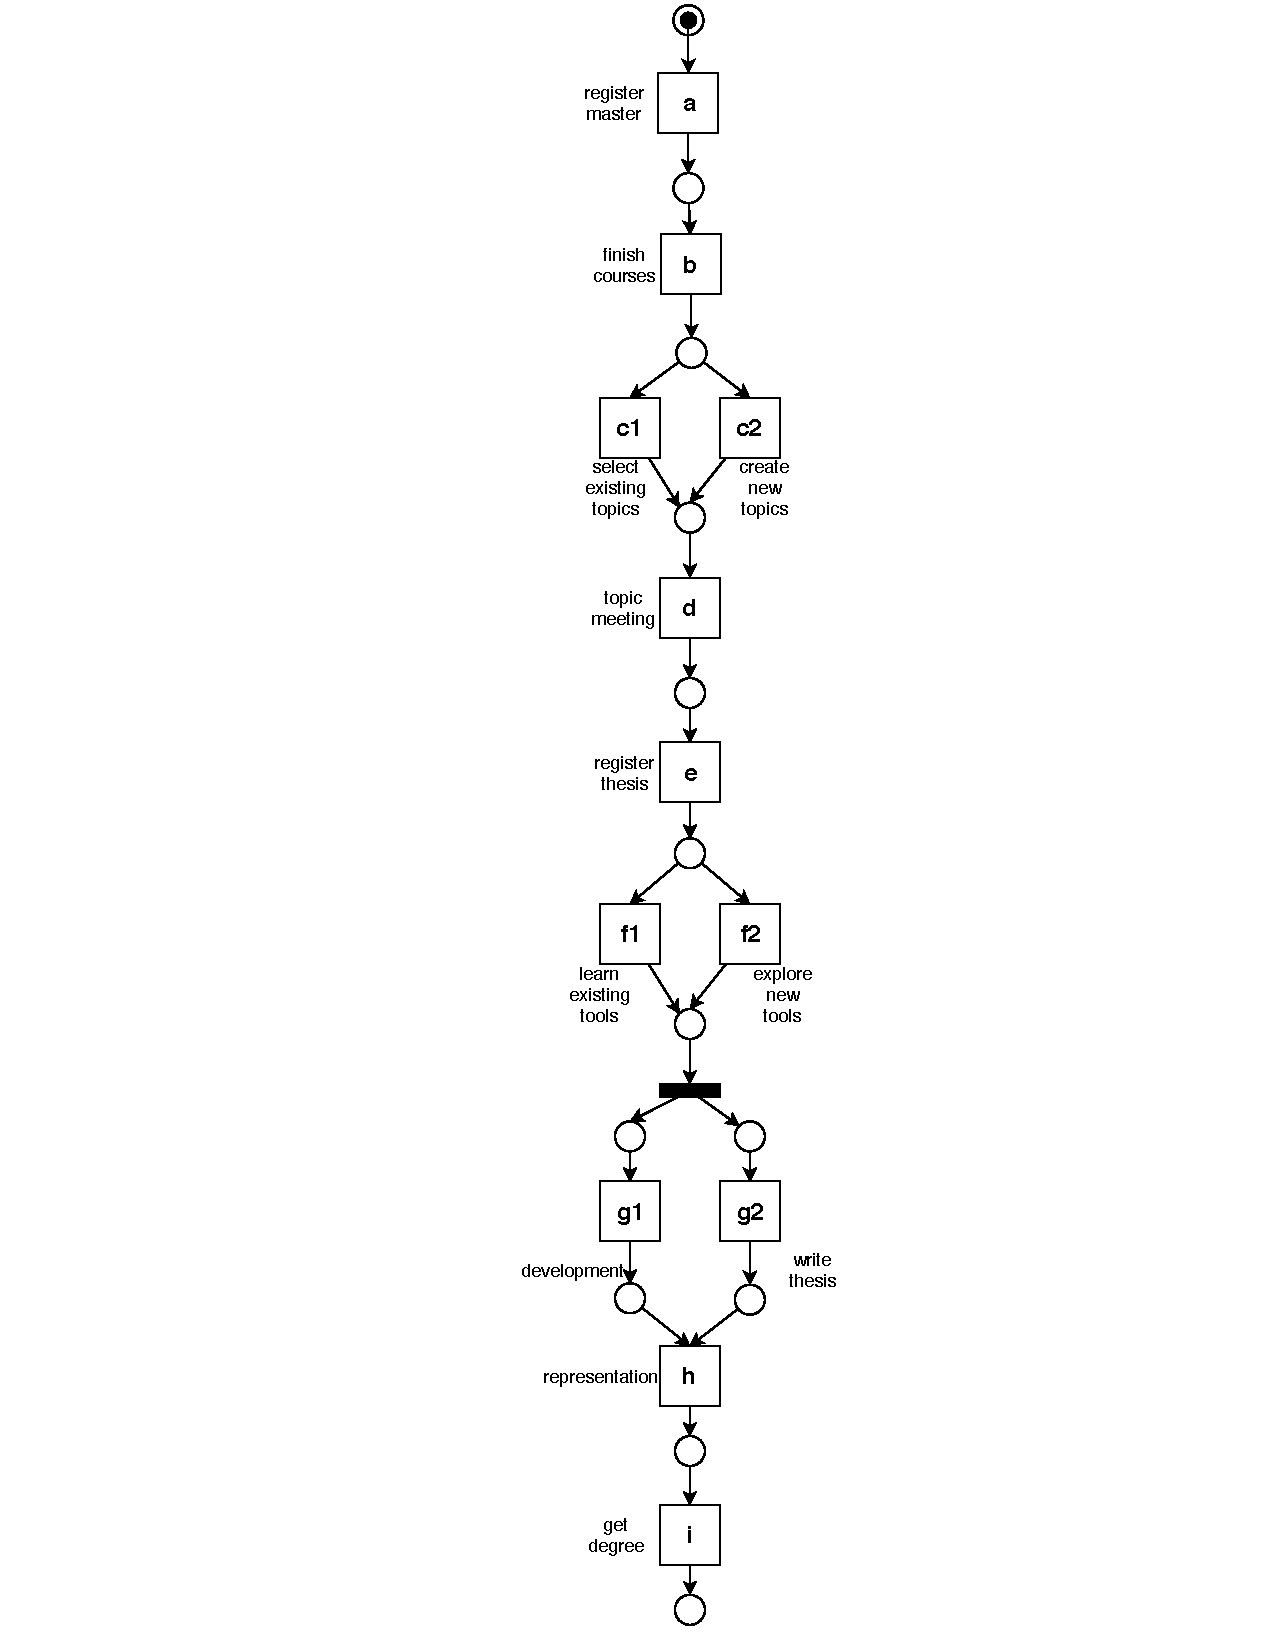
\includegraphics[clip, trim=8cm 0cm 8cm 0cm, width=0.5\linewidth, height=0.7\textheight]{figures/introduction/Master-change-order.pdf}
		\caption{expected model $M_{2}$ with order change}
		\label{fig:model_c}
	\end{subfigure}%
	\begin{subfigure}[b]{0.5\textwidth}
		\centering
		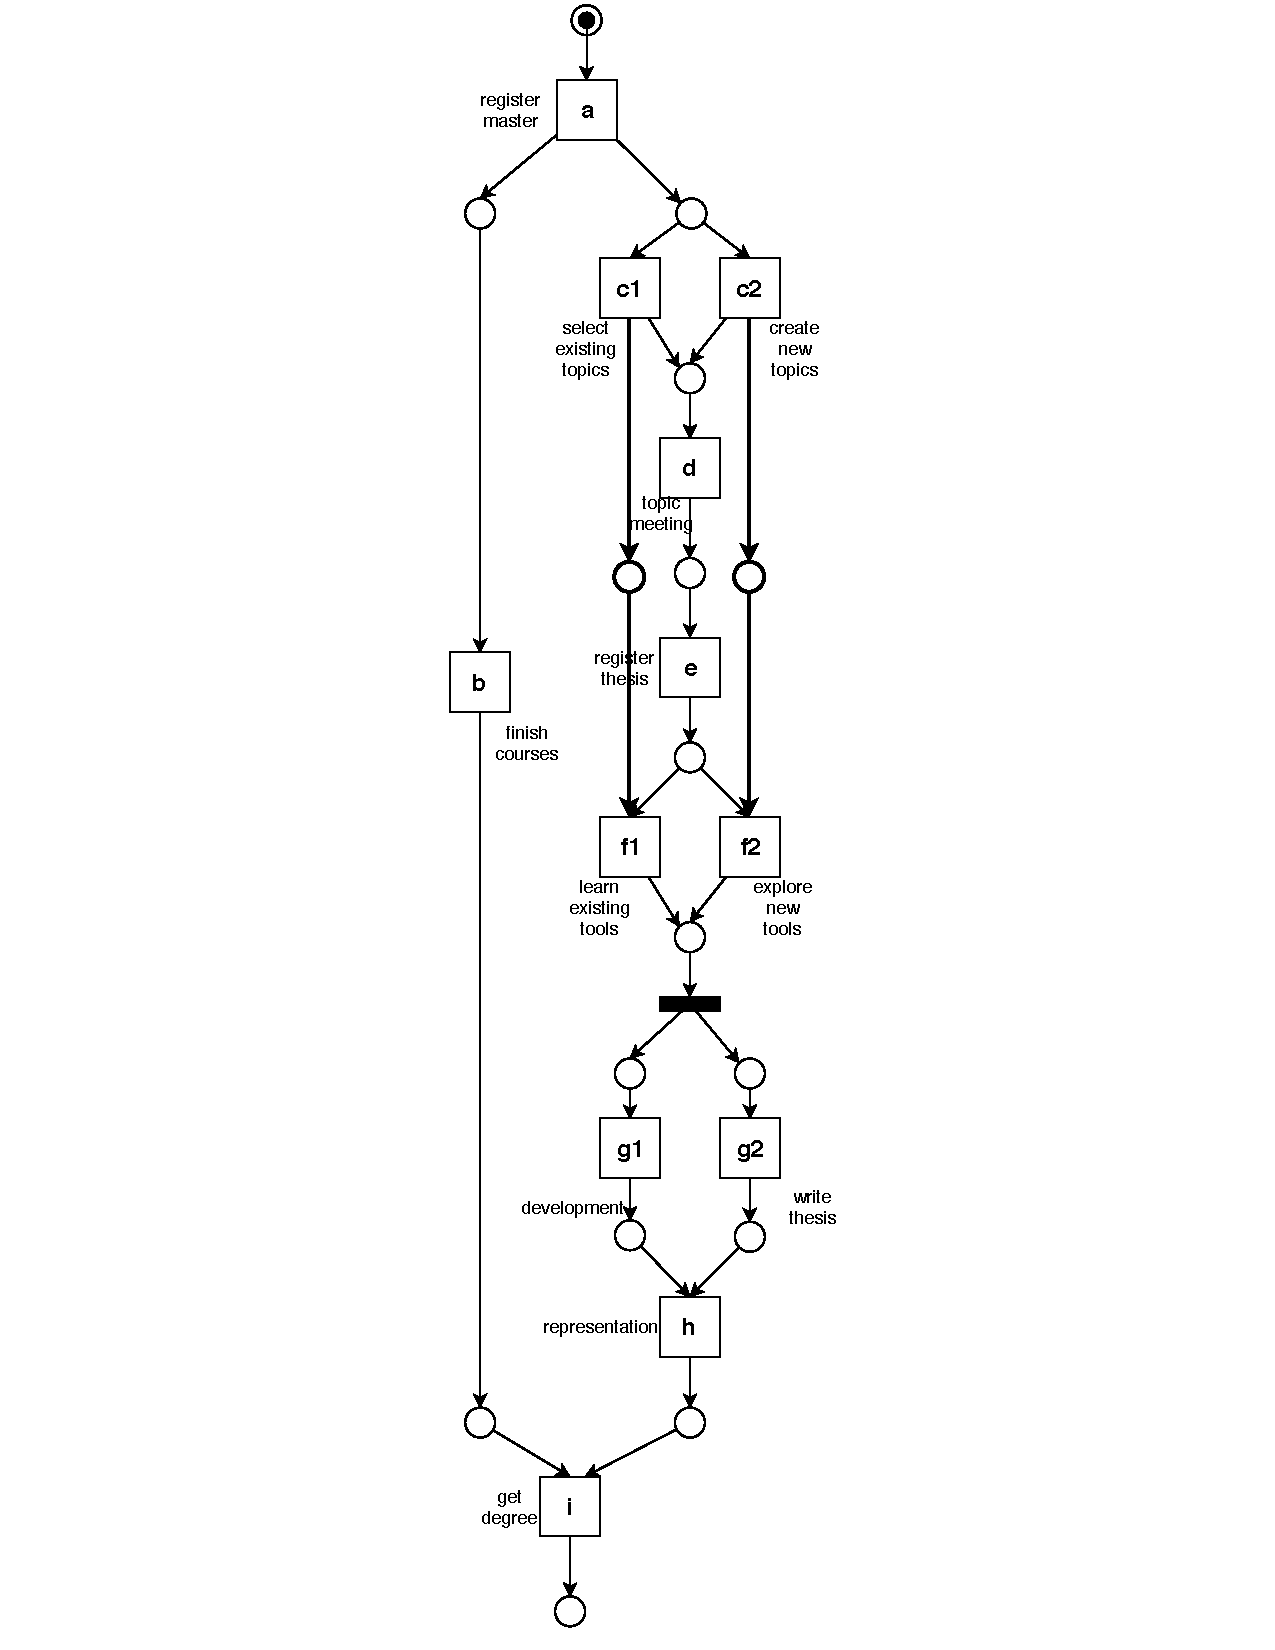
\includegraphics[clip, trim=7cm 0cm 7cm 0cm, width=0.5\linewidth, height=0.7\textheight]{figures/introduction/Master-with-lt.pdf}
		\caption{model $M_{3}$ with long-term dependency}
		\label{fig:model_d}
	\end{subfigure}
	\caption{example for situation 2 and 3}
	\label{fig:model_changes_2_3}
\end{figure}
\subsection{Situation 3: \small{detect long-term dependency}}
This part introduces a problem which causes a lower precision in process mining. It is the inability in current methods to detect the long-term dependency in the Petri net. The long-term dependency describes the phenomenon that one execution choice decides the execution of activities that do not follow directly. Due to the long distance of this dependency, current methods cannot detect it and improve the precision by adding long-term dependency on the model. 
An event log $L_3$ is given in the following. By using time consumption as one KPI, if the total sum goes over one threshold, we mark this trace as negative, else as positive. Since the activity \emph{create new topics} usually demands new knowledge rather than checking the existing tools. So if students choose to learn existing tools, it's possibly not useful and time is wasted. In the other case, if we select existing topics with existing background, it saves time when we directly learn the existing tools. According to this performance standard, we classified those event traces.
\emph{Event Log $L_3$ -- }
\begin{align*}
Positive:\{ & { <a,b,\textbf{c1},d,e,\textbf{f1},g1,g2, h,i>}^{50}, \\   &{<a,b,\textbf{c2},d,e,\textbf{f2},g2,g1, h,i>}^{50} \}  \\
Negative: \{ & {<a,b,\textbf{c1},d,e,\textbf{f2},g2,g1,h,i>}^{50}, \\
& {<a,b,\textbf{c2},d,e,\textbf{f1},g1,g2,h,i>}^{50}  \}
\end{align*}
%here we list one example to explain the long-term dependency, but we need to make them clear, might without the loop item..It means that we need to change the whole model..
There are no deviations of the model and event log $L_3$ according to the  algorithms in \cite{fahland2015model} and \cite{dees2017enhancing}. Therefore, the original model stays the same and allows for the execution of negative instances. After checking the model and log, those long-term dependencies have significant evidence. Transition \textbf{\emph{c1}} decides \textbf{\emph{f1}} while \textbf{\emph{c2}} decides \textbf{\emph{f2}}.  After addressing long-term dependency like the model $M_3$ in Figure \ref{fig:model_d} by connecting transitions to extra places, 
negative instances are blocked and the model has higher precision.

Clearly, the use of negative information can bring significant benefits, e.g, enable a controlled generalization of a process model: the patterns to generalize should never include negative instances. The demand to improve current repair model techniques with incorporating negative instances appears. In the next section, the demand is analyzed and defined in a formal way.

\section{Research Scope And Questions }
After analyzing the current model repair methods, we limit our research scope as shown in Figure \ref{fig:scope}.  The inputs for our research are one existing process model M, an event log L . According to predefined KPIs, each trace in event log is classified into positive or negative. After applying repair techniques in the black box, the model should be improved to enforce the positive instances while disallowing negative instance, with condition that the generated model should be as similar to the original model as possible. 
\begin{figure}
	\centering
	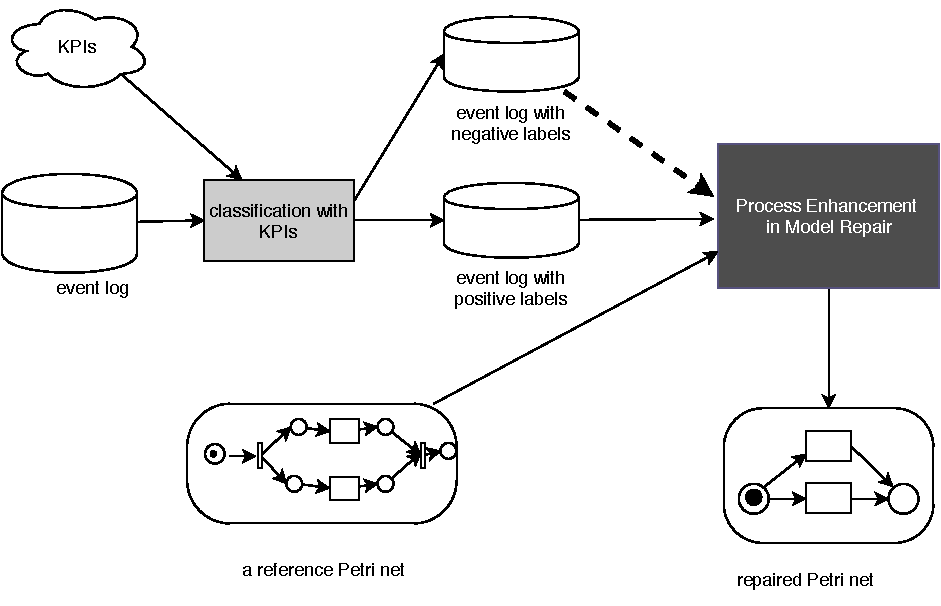
\includegraphics[width=\textwidth]{figures/introduction/P06-problem-scope.pdf}
	\caption{The problem description}
	\label{fig:scope}
\end{figure}

In this scope, we come up with several research questions listed in the following.
\begin{enumerate}[start=1,label={\bfseries{ RQ\arabic*:}}]
	%\itemsep0em
	\item How to overcome the shortcomings of current repair techniques in situations 1-3 above?
	\item How to balance the impact of the existing model, negative and positive instances together to repair model? 
	\item How to block negative instances from the model while enforcing the positive ones?
\end{enumerate}
  
In the remainder, we propose a solution for the black box. It analyzes process performance on trace level and balances the existing model, positive traces and negative traces on directly-follows relation, in order to incorporate all the factors on model generation. 

\section{Outline}
This thesis tries to answer the questions presented in section 1.2 in the remainder chapters and provide a solution for the black box. 
Chapter 2 and 3 introduces the related work and recalls the basic notions on process mining and list the preliminary to solve the problem. 
Chapter 4 describes the algorithm to solve the problem. 
In Implementation part, screenshots are given from the finished tools of our algorithm to demonstrate the use.  Experiment chapter answers the last question RQ3, by conducting a bundle of experiments. Later, results are analyzed and discussed. 
The last chapter is the summary of our work. 
%The next section answers the questions, how to balance all factors and block negative instances, Our algorithm analyzes process performance on trace level and balances the existing model, positive traces and negative traces on directly-follows relation, in order to incorporate all the factors on model generation. Long-term dependency is further detected on the intermediate model and added to block negative instances. What's more, the impact of the existing model, positive and negative instances are parameterized by weights, to allow more flexibility of the generated model.



%\end{document}

\chapter{Preliminaries} \label{chap:prelim}
\subsection{Definitions Related To Dfg-Method}
In this part, we provides concepts related to the dfg-method which is based on directly-follows graph. A directly-follows graph as used in \cite{leemans2013discovering}, represents the directly-follows relation of activities in event log. For instance, if there are traces of $\langle ...,A,B,... \rangle$ in event log, one edge (A,B) is added into directly-follows graph. By cutting directly-follows graph under different conditions, Inductive Miner\cite{leemans2013discovering,leemans2014discovering} discovers a process model. Unlike this process, we adapt Inductive Miner to repair model by using existing model, and event log with labels.

\begin{definition}[Cardinality in directly-follows graph]
	Given a directly-follows graph G(L) derived from an event log L, the cardinality of each directly-follows relation in G(L) is defined as:  
	\begin{itemize}
		\item $Cardinality(E(A,B))$ is the frequency of traces with $\langle ...,A,B,... \rangle$. 
		\item Start node A cardinality $Cardinality(Start(A))$ is the frequency of traces with begin node A.
		\item End node B cardinality $Cardinality(End(A))$ is the frequency of traces with end node B.
	\end{itemize}	
\end{definition}
From the positive and negative event log, we can get directly-follows graphs, respectively $G(L_{pos})$ and $G(L_{neg})$. Each edge of  $G(L_{pos})$ and $G(L_{neg})$ has a cardinality to represent the strength of this directly-follows relation. 
However, when the existing model is transformed into  directly-follows graph $G(L_{ext})$, there is no point to assign cardinality on each edge. So we just set 1 to cardinality of each edge. 

%To incorporate all information from  $G(L_pos)$, $G(L_neg)$ and $G(L_ext)$, a data structure is defined directly-follows matrix. 
To incorporate all information from  $G(L_{pos})$, $G(L_{neg})$ and $G(L_{ext})$, we define  weight for each directly-follows relation in graph. 
\begin{definition}[Weight of directly-follows relation]
	Given a directly-follows graph G(L), the weight of each directly-follows relation is defined as \[ Weight(E(A,B)) = \frac{Cardinality(E(A,B))}{Cardinality(E(A,*))}  \] 
	for start activities A, we have 
	\[ Weight(Start(A)) = \frac{Cardinality(Start(A))}{Cardinality(Start(*))} \]
	Similarly for end activities B, we have
	\[ Weight(End(B)) = \frac{Cardinality(End(B))}{Cardinality(End(*))} \]
	E(A,*) means all edges with source A, E(*,B) means all edges with target B, Start(*) represents all start nodes, and End(*) represents all end nodes.
\end{definition}
After defining the weights of each directly-follows relation, for each directly-follows relation, there are three weights from $G_{pos}$, $G_{neg}$ and $G_{ext}$. The following strategy assigns new weight to directly-follows relation to new generated directly-follows graph $G_{new}$.
\begin{definition}[Assign new weights to graph $G_{new}$]
	there are three weights from $G_{pos}$, $G_{neg}$ and $G_{ext}$, the new weight is 
	\begin{itemize}
		\item For one directly-follows relation, \[ Weight(E_{G_{new}}(A,B)) = Weight(E_{G_{pos}}(A,B)) + Weight(E_{G_{ext}}(A,B)) - Weight(E_{G_{neg}}(A,B))\]
		\item For start activities A, we have 
		\[ Weight(Start_{G_{new}}(A)) = Weight(Start_{G_{pos}}(A)) + Weight(Start_{G_{ext}}(A)) - Weight(Start_{G_{neg}}(A)) \]
		\item For end activities B, we have
		\[ Weight(End_{G_{new}}(A)) = Weight(End_{G_{pos}}(A)) + Weight(End_{G_{ext}}(A)) - Weight(End_{G_{neg}}(A)) \]
	\end{itemize}
\end{definition}
After assigning all the weight to directly-follows relation in $G_{new}$, we filter out all directly-follows relation in $G_{new}$ with weight less than 0. 
Then, we transform the $G_{new}$ into process tree bu using Inductive Miner for the next stage.

\subsection{Definitions Related To Add Long-term Dependency}
\textit{Example 1} Consider event log L with labels \[L =[\langle A,C,E \rangle^{50,pos}, \langle B,C,D \rangle^{50,pos}, \langle A,C,D \rangle^{50,neg}]. \] $\langle A,C,E \rangle^{50,pos}$ means there are 10 traces $\langle A,C,E \rangle$ labeled as positive in event log. Similarly, $\langle A,C,D \rangle^{50,neg}$ represents there are $\langle A,C,D \rangle$ traces at number 50 in event log which have negative labels. 

After applying the dfg-algorithm, a model as shown in Figure \ref{fig:pn_without_lt_exm01} is discovered. In event log L, B and D has long-term dependency, and A is expected to support only the execution of E, since $<A,C,D>$ is negative and $<A,C,E>$ is positive. However, the model doesn't express those constraints.
\begin{figure}[h!]
	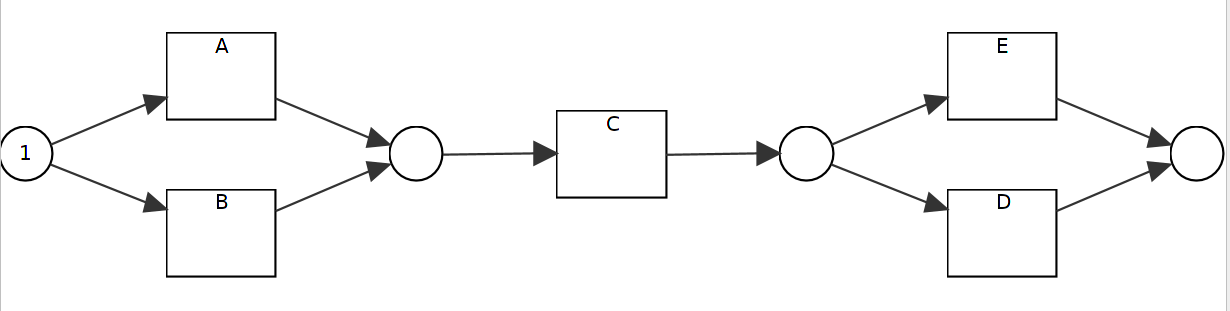
\includegraphics[width=\textwidth]{figures/preliminaries/PN06_Seq_2_xor_notnested.png}
	\caption{Process model generated from dfg-algorithm}
	\label{fig:pn_without_lt_exm01}
\end{figure}
Obviously, long-term dependency relates the choices structure in process model, such as exclusive choice, loop and or structure. Due to the complexity of or and loop structure, only the long-term dependency in exclusive choice is considered. 

The inputs for this algorithm are,
\begin{itemize}
	\item Repaired model in process tree
	\item Event log with positive and negative labels
\end{itemize}
The output of this algorithm is: 
\begin{itemize}
	\item Repaired model in petri net with long-term dependency
\end{itemize}
%%if now, we only consider the repaired process tree model, then we don't have problems to make the weights of dfg and long-term dependency unified. But we have it from the existing model, because of existing factor. 
%% Now we have the firstly-repaired model, if we want to create long-term dependency, we also have the 3 weights:: 
%% Ext_Wlt(Si, Tj), but when our negative factor affects, we need to unify them!!To prove it!!! 

Process tree, as one input for the algorithm, is one common model to interpret business process in process mining. It's a block-structured tree. To specify the process tree with respect to long-term dependency, the following definitions are in need. Firstly, the definitions related to tree are reviewed.
\begin{definition}[Tree]
	Let $ \mathscr{E} $ be a finite set of entities, a tree is a collection of entities called nodes, which are connected by edges. A tree T is,
	
	\begin{itemize}
		\item t, with  $t\in \mathscr{E}$, t has no outgoing edges
		\item $t(T_1,T_2,...,T_n)$, with $t\in \mathscr{E}, i,n\in \mathbb{N}, i \leq n ,T_i$ is a tree.
	\end{itemize}
\end{definition}
$T_i$ is a child or subtree of $t(T_1,T_2,...,T_n)$, $t(T_1,T_2,...,T_n)$ is one parent of $T_i$, which can be expressed in $P(t(T_1,T_2,...,T_n),T_i)$. The root of tree is the node without any parent; A tree has only one root. A leaf node is the node which has no children nodes.\\
For a node in a tree, its ancestor and descendant are defined as:
\begin{definition}[Ancestor Relation Anc(A,t)]
	An ancestor of a node t in a tree is a node A, written as $ Anc(A,t) \Rightarrow True$, if those conditions hold,  
	\begin{itemize}
		\item A is a parent of t, written as $ P(A,t) \Rightarrow True$, or
		\item $\exists t_1,t_2..t_n,n\in \mathscr{E}, i < n, P(A,t_1)\land P(t_i,t_{i+1}) \land P(t_n,t) \Rightarrow True $
	\end{itemize}
\end{definition}
The ancestor of root is empty, while leaf nodes has no descendants. Based on this, we define the ancestors set of a node s. 
\begin{definition}[Ancestors of a node a]
	The ancestors set of a node s, Ancestors(s), is defined as: \[ Ancestors(A)=\{t|Anc(t,s) \Rightarrow True \} \]
\end{definition}
Accordingly, descendant relation is given for node t and node s, Des(s,t). If node s is the ancestor of t, then t is a descent of s. $Anc(s,t) \Rightarrow Dec(t,s)$; The set of descendants of node t is Descendants(t).
\begin{definition}[Least Common Ancestor]
	A least common ancestor for node $s$ and node $t$ in a tree is a node n, where 
	\[Anc(n,s) \land Anc(n,t) \land \exists! m Anc(n,m) \land Anc(m,s) \land Anc(m,t) \]
\end{definition}

In process tree, all the leaves are activities in business process, and the middle nodes are operators which represents the relations of all its children nodes\cite{vanderAalst:2016:PMD:2948762,leemans2013discovering}. This paper uses four operators in context of long-term dependency. The four relations.  $\{\rightarrow, \times, \land, \circlearrowright\}$ are considered. 

Next, we only focus on exclusive xor structure on long-term dependency. As known, long-term dependency is associated with choices. In xor block, it means the choices of each xor branch in xor block. For sake of convenience, we define the xor branch.

$Q= \times(Q_1 , Q_2 ,.. Q_n)$, $Q_i$ is one xor branch with respect to Q, rewritten as $XORB_{Q_i}$ to represent one xor branch $Q_i$ in xor block, and record it $XORB_{Q_i} \in XOR_{Q}$. For each branch, there exists the begin and end nodes to represent the beginning and end execution of this branch, which is written respectively as Begin($XORB_{Q_i}$) and End($XORB_{Q_i}$).

%% but the structure of xor branch, do we need to think of right now?? we need to think of it 
For convenience of analysis, two properties of xor block, purity and nestedness are demonstrated to express the different structures of xor block according to its branches.
\begin{definition}[XOR Purity and XOR Nestedness] The xor block purity and nestedness are defined as following: \\
	\begin{itemize}
		\item A xor block $XOR_Q$ is pure if and only $\forall XORB_X \in XOR_Q, XORB_X $ has no xor block descent, which is named as pure xor branch. Else,
		\item A xor block $XOR_Q$ is nested if $ \exists XOR_X, Anc(XOR_Q, XOR_X) \rightarrow True  $. Similarly, this xor branch with xor block is nested.
	\end{itemize}
\end{definition}
%% change the graph for whole explaination!!
In the Figure\ref {fig:xor_nested_branch_variants}, xor block Xor(c1,c2) are pure and not nested, since all the xor branches are leaf node, but xor block Xor(a,Seq(b,Xor(c1,c2))) is impure and nested with Xor(c1,c2). 
\begin{figure}[h!]
	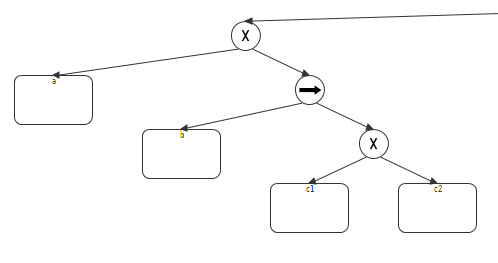
\includegraphics[width=\textwidth]{figures/preliminaries/PT02_xor_nested_and_pure.png}
	\caption{XOR branch variants}
	\label{fig:xor_nested_branch_variants}
\end{figure}

%% xor branch, the dependency between them, then how about the dependency on that part, does it exist in the xor block, so we can define it ??
%% the full completeness is also dependency, but sth different, 
%% for arbitrary two xor branches, if they are long-term dependency?? Can I decide, or not ?? I can decide it!! But in the specific way, if they are in a pair, they are ok, else, not !!! 
%% but it goes far, so only write down what I have achieved, but in their thinking way, why in my way?? 
%% given two branch, and they have order, just complexity of implementation, then we only consider the directly ones!!  

Long-term dependency researches on the dependency of choices in xor block, with observation, actually on the pure xor branch, because nested xor branch has multiple choices, which affect the execution of later process. For two arbitrary pure xor branches, to have long-term dependency, they firstly need to satisfy the conditions: (1) they have an order;(2) they have significant correlation.
The order of xor branch follows the same rule of node in process tree which is explained in the following.
\begin{definition}[Order of nodes in process tree]
	Node $X$ is before node $Y$, written in $X \prec Y$, if $X$ is always executed before $Y$.  In the aspect of process tree structure, $X \prec Y$, if the least common ancestor of $X$ and $Y$ is a sequential node, and $X$ positions before $Y$.
\end{definition} 
%% how to define the correlation fo xor branches, if they always happen together
The correlation of xor branches is significant if they always happen together. To define it, several concepts are listed at first. 
\begin{definition}[Xor branch frequency]
	Xor branch $XORB_X$ frequency in event log l is $F_{l}(XORB_X)$, the count of traces with the execution of $XORB_X$. \\
	For multiple xor branches, the frequency in event log l is defined as the count of traces with all the execution of xor branches $XORB_{Xi}$ , written as \[F_{l}(XORB_{X1}, XORB_{X2},...,XORB_{Xn})\].
\end{definition}
%% correlation means the two always happen together, if one not shown, the other also not?? So the connection support.. how to define them?? 
%% connection support, we can say only on number, when it is over one value, 
After calculation of the frequency of the coexistence of multiple xor branches in positive and negative event log, we get the supported connection of those xor branches, and define the correlation. 
\begin{definition}[Correlation of xor branches]
	\label{def: supported-connection}
	For two pure xor branches, $XORB_X \prec XORB_Y$, the supported connection is given as \[SC(XORB_X,XORB_Y)= F_{pos}(XORB_X, XORB_Y) -F_{neg}(XORB_X, XORB_Y)\]. If $SC(XORB_X,XORB_Y) > lt-threshold$, then we say $XORB_X$ and $XORB_Y$ have significant correlation.
\end{definition}

I did some introduction, it is proven that in some cases, we can't deal with it. When the $XORB\_S \neq LT\_S || XORB\_T \neq LT\_T$.

Another way to avoid this problem is to add duplicated events, but the problem stays the same, so if we want to keep the model fit, we add new event for the discovered long-term dependency, the original, we keep it in the model?? But it is not precise!!! It allows too many choices there, but the model is sound, because we add events on model, we produce and consume tokens from duplicated events, and consumes it later.. Still, it is not so right. But if we choose the events before, we decides the events later, it's true... helps a little... 

How to prove it ?? By induction. 
We use  process  trees as one internal result in  our  approach in two factors: (1) they are sound by construction, and can be transferred into sound Petri net models; (2) they are block-structured. which benefits the detection of exclusive relations in model.

\begin{itemize}
	\item the original model is sound
	\item after adding one long-term dependency by duplicating the event, we make sure
	 \\ duplicated events are added into the xor branches, if it's chosen, then it consumes one token, at this xor branches, then it produces two tokens, one of which is put back again into the 
	 To prove the added places and duplicated events between two xor branches will not violate the soundness of model. 
	 \item 
	 \begin{itemize}
	 	\item adding duplicated events of one long-term dependency does not violate the soundness of model. 
	 	
	 	\item To connect the source and target  of long-term dependency which are the duplicated events will not violate the soundness.
	 	\\ One extra place is added to connect the source and target. After executing the source, one token is generated in this place; Due to long-term dependency, only this target is triggered by this token and it consumes this token. No extra token is introduced into this model, so the model keeps sound. 
	 	
	 \end{itemize}
	 
	 \item While keeping the original event in the model,  the model is with less precision.  
	 \\ 
	 So I want to solve this problem, and make it preciser by considering the original events into model... 
	 One drawback exists there, still... If we use the old and then the 
\end{itemize}

It's about 12 pages. But one problem, some basic information, we forget to give .. Maybe, we can put the related work later!!!



\chapter{Approach} \label{chap:appr}
Analyzing conformance and performance expressed as averages over the whole model and log is very broad. Many real-life processes contain complex patterns and behavior as shown in the introduction. They can only be discovered when combining multiple perspectives on the data. The approach presented here focuses on localizing metrics for conformance, performance and process context to individual places in the Petri net model. The metrics are further localized to time intervals to make changes over time visible.

The approach consists of three steps:
\begin{enumerate}
    \item The log is projected onto the places of the process model to extract a \emph{locally mapped log}
    \item \emph{Interactions} are extracted from this \emph{locally mapped log}
    \item Metrics are calculated from \emph{interactions} for time intervals
\end{enumerate}

In the following, we introduce these steps in order.

\section{Locally mapping the log}
The first step requires some pre-processing. To properly handle the start and end places in the next steps, we insert unique start and end events into every trace. Their $activity$ is $\tstart$ or $\tend$ respectively. Their $time$ attribute is the time of first or last event respectively. Let $\E^\prime \supset \E$ be the universe of events including all artificial start and end marker events. To add the corresponding $\tstart$ and $\tend$ transitions in the model, a system net $SN=(PN,M_i,M_f)$ with initial and final marking is required. The $\tstart$ transition $t_{\tstart}$ is connected to all places in $M_i$ and the $\tend$ transition $t_{\tend}$ from all places in $M_f$. So for $PN = (P,T,F,l)$ the pre-processed Petri net is $PN^\prime=(P,T^\prime,F^\prime,l^\prime)$ with $F^\prime = F \cup \set{ (t_{\tstart},p) }{p\in M_i}\cup \set{(p,t_{\tend})}{p \in M_f}$, $T^\prime = T \cup \{t_{\tstart},t_{\tend}\}$, $\forall t\in T: l^\prime(t)=l(t)$ and $l^\prime(t_{\tstart}) = \tstart, l^\prime(t_{\tend})) = \tend$. Figure \ref{fig:preprocessednet} shows the pre-processed version of Figure \ref{fig:simplenet}.

\begin{figure}
    \centering
    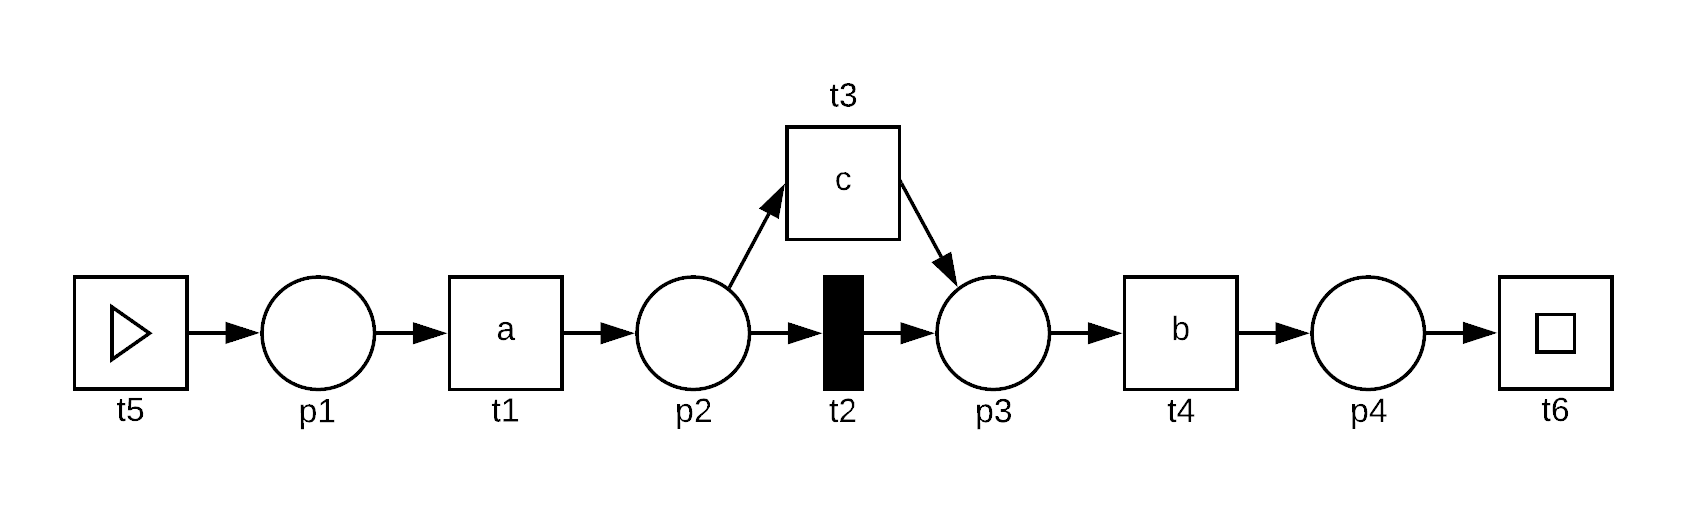
\includegraphics[width=0.6\textwidth]{figures/concept/preproc_simplenet.png}
    \caption{The simple model after pre-processing}
    \label{fig:preprocessednet}
\end{figure}

From this point on, we assume all Petri nets and logs to be pre-processed in this way.
We partition the adjacent transitions of a place into visible and invisible transitions, so for a place $p\in P$, $adj(p)=(\pre p \cup \post p) \cap T^{l}$ is the set of adjacent visible transitions and $adj_{\tau}(p) =(\pre p \cup \post p) \cap T^{\tau}$ is the set of adjacent silent transitions. To be able to add silent transition executions, let $l_{\tau}:T^{\tau} \to A_{\tau}$ be a labeling function which assigns a unique artificial activity to every otherwise unlabeled $\tau$-transition. To further define the silent execution events, let $\I$ be the universe of all artificial silent (hence not in $\E^\prime$) events whose $activity$ attribute is a silent activity. With these definitions, a locally mapped case can be defined. It is a mapping of events from a case to transitions adjacent to a particular place.
\begin{definition}[Locally mapped case]
Let $\Log \in \Univ L$ be a log and $PN = (P,T,F,l)$ be a Petri net. For a case $c\in \Log$ and place $p\in P$, a locally mapped case $lmc$ for $p$ inherits (and overloads) all attributes of $c$ except for the $trace$ attribute. Its trace is overloaded to a sequence of pairs of real events from $\hat{c}$ and inserted artificial silent events together with a fitting transition, i.e. $\hat{lmc}=trace(lmc)\in ((\E^\prime \times adj(p)) \cup (\I \times adj_{\tau}(p)))^*$. For every pair $(e,t)\in \E^\prime \times adj(p)$ or $(i,t^\prime)\in \I \times adj_{\tau}(p)$ in the sequence, the label of the transition has to match the activity of the event, i.e. $activity(e) = l(t)$ and $activity(i) = l_{\tau}(t^\prime)$. All events in the sequence have to be unique and ordered by $time$, so $\forall 1\le i<j \le |\hat{lmc}|, \hat{lmc}_i=(e,t), \hat{lmc}_j = (e^\prime,t^\prime): e\neq e^\prime \wedge time(e) \le time(e^\prime)$. Lastly, the projection onto real events is a subset of the original trace, i.e. $set(\hat{lmc}\restriction_1\restriction_{\E^\prime}) \subseteq set(\hat{c})$. If $|\hat{lmc}| = 0$, $lmc$ is called an empty locally mapped case which means the case did not interact with the place $p$.
\end{definition}
There are many ways to map a case onto the locally mapped cases, so we first define a generalized strategy. The strategy also determines the mandatory $time$ attribute of inserted silent events.
\begin{definition}[Case mapping strategy]
Let $\Log \in \Univ L$ be a log and $PN = (P,T,F,l)$ a Petri net. For any case $c\in \Log$, a case mapping strategy $\func{case\_map\_strat(c)} = (lmc_p)_{p \in P}$ creates a locally mapped case for each place $p\in P$. It needs to be consistent because a transition execution mapped in one of the locally mapped cases needs to be included in all the others also adjacent to the transition. So, $\forall p\in P \ \forall (e,t) \in set(\hat{lmc}_p) \ \forall p^\prime \in (\pre t \cup \post t): (e,t)\in set(\hat{lmc}_{p^\prime})$.
\end{definition}
Consistency can be achieved by first selecting a subset of events, mapping them to transitions, adding silent executions and then projecting them onto the adjacent transitions of the places.
Now, the entire event log can be mapped onto individual places with locally mapped logs.
\begin{definition}[Locally mapped log]
Let $\Log \in \Univ L$ be a log, $PN = (P,T,F,l)$ be a Petri net and $\func{map\_strat}$ be a case mapping strategy. Then a locally mapped log $\Log_p$ of place $p\in P$ is the set of all non-empty locally mapped cases, i.e. $\Log_p=\set{lmc}{lmc = \func{map\_strat(c)}_p \wedge |\hat{lmc}|\neq 0 \wedge c \in \Log }$.
\end{definition}

We propose a specific case mapping strategy $\func{sync\_strat}$ where a global execution is mapped locally. It uses alignments to be able to handle duplicate transitions and silent transition executions. 
The synchronous moves already provide a mapping of a subset of events from the trace to transitions in the model, so only the silent transition executions have to be added. This is done by replaying the synchronous and invisible moves on the model in a token-based manner. Synchronous moves are always executed, even if not enabled. Invisible moves are only executed if they are enabled, to be able to set their $time$ attribute which is the instant they are enabled. That means chains of silent events consistently shift the sojourn duration between two real events to the place at the end of the chain. The invisible move chains can be cut-off by non-invisible model moves, leaving the deviation of missing this event on the places adjacent to these non-invisible model moves.
This way, the locally mapped cases can be seen as a projection of the fitting parts of the event log onto locally mapped logs for each place.
A variant $\func{all\_strat}$ also tries to consider log moves which makes it unsuitable for models with duplicate transitions. It essentially treats log moves which can be mapped to a transition as synchronous moves, executing them unconditionally. More information from the log is used that way. Especially loops in a trace which cannot be mimicked by the model and hence end up being log moves can contribute to the analysis this way.

\begin{algorithm}[tb]
\begin{algorithmic}
\Require given $PN = (P,T,F,l)$
\State $\forall p\in P: lmc_p \gets$ new locally mapped case
\State $\forall p\in P: \hat{lmc}_p \gets \langle \rangle$
\State $M \gets$ new empty marking
\State $\var{lastMappedTime}: P \nrightarrow Time$
\Function{mapStrat}{alignment $\gamma$, boolean $\var{mapLogMoves}$}
    \For{$i = 1 : |\gamma|$}
        \If{$\gamma_i = (e,t) \wedge activity(a) = l(t)$} \Comment{sync move}
            \State \Call{handleTransition}{$e$, $t$}
        \ElsIf{$\gamma_i = (e, \gg)$} \Comment{log move}
            \If{$\var{mapLogMoves} \wedge \exists t\in T: l(t) = activity(e)$}
                \State \Call{handleTransition}{$e$, $t$}
            \EndIf
        \ElsIf{$\gamma_i = (\gg, t) \wedge l(t) = \tau$} \Comment{inv move}
            \If{$M[t\rangle$}
                \State $enabledAt \gets \max\{ \var{lastMappedTime}(p)| p\in \pre t \}$
                \State $e_{\tau} \gets$ new unique event
                \State $activity(e_{\tau}) \gets l_{\tau}(t)$
                \State $time(e_{\tau}) \gets enabledAt$
               \State \Call{handleTransition}{$e_{\tau}$, $t$}
            \EndIf
        \EndIf
    \EndFor
    \State \Return $(lmc_p)_{p\in P}$
\EndFunction
\Function{handleTransition}{event $e$, transition $t$}
    \State $M \gets (M \setminus \pre t) \uplus \post t$
    \ForAll{$p \in {\pre t \cup \post t}$}
        \State $\hat{lmc}_p \gets \hat{lmc}_p \cdot (e,t)$
        \If{$p \in \post t$}
            \State $\var{lastMappedTime}(p) \gets time(e)$    
        \EndIf
    \EndFor
\EndFunction
\end{algorithmic}
\caption{The proposed $\func{map\_strat}$}
\label{alg:mapstrat}
\end{algorithm}

A configurable algorithm for both variants is presented in Algorithm \ref{alg:mapstrat}. Provided an alignment $\gamma$ of a case, it steps through the sequence of moves and updates the locally mapped cases accordingly in the helper function \textsc{handleTransition}. It uses the partial function $\var{lastMappedTime}$ to track timestamps and a marking $M$ as an updated current marking. The transitions of synchronous moves and, if desired, mapped log moves are fired regardless if they are enabled. Invisible model moves are executed if they were actually enabled otherwise they are ignored. When they are executed, a unique new event is created and its mandatory attributes set. Then it is treated like any other transition execution.

As an example, consider the pre-processed log cases $\hat{c_1} = \langle e_{11}^\tstart, e_{12}^b, e_{13}^a, e_{14}^c, e_{15}^\tend \rangle$ and $\hat{c_2} = \langle e_{21}^\tstart, e_{22}^a, e_{23}^b, e_{24}^\tend \rangle \}$ in log $\Log = \{ c_1, c_2\}$ on the model given in Figure \ref{fig:preprocessednet}. The results of both strategies on this log are shown in Figure \ref{fig:mapstrats}. With $\func{sync\_strat}$, the unfitting event $e_{12}^b$ of the first case is not mapped which assigns that deviation to places $p3$ and $p4$. $\func{all\_strat}$ maps this event, which hides the problem from $p4$ and focuses it on $p3$ as swapped events.
\begin{figure}
    \centering
    \begin{tabular}{|l|c|}
    \hline
    Local log & $\func{sync\_strat}$  \\
    \hline
    $\Log_{p1}$ 
    & $\{ \langle (e_{11}^\tstart,t5),(e_{13}^a,t1) \rangle, \langle (e_{21}^\tstart,t5), (e_{22}^a,t1) \rangle \}$ 
     \\
    $\Log_{p2}$ 
    & $\{ \langle (e_{13}^a,t1), (e_{14}^c,t3) \rangle, \langle (e_{22}^a,t1),(e_{\tau}^{t2},t2) \rangle \}$ 
    \\
    $\Log_{p3}$ 
    & $\{ \langle (e_{14}^c,t3) \rangle, \langle (e_{\tau}^{t2},t2),(e_{23}^b, t4) \rangle \}$ 
    \\
    $\Log_{p4}$ 
    & $\{ \langle (e_{15}^\tend, t6) \rangle, \langle (e_{23}^b,t4),(e_{24}^\tend, t6) \rangle \}$ 
    \\
    \hline
    \hline
    Local log & $\func{all\_strat}$ \\
    \hline
    $\Log_{p1}$ & $\{ \langle (e_{11}^\tstart,t5),(e_{13}^a,t1) \rangle, \langle (e_{21}^\tstart,t5), (e_{22},a) \rangle \}$ \\
    $\Log_{p2}$ & $\{ \langle (e_{13}^a,t1), (e_{14}^c,t3) \rangle, \langle (e_{22}^a,t1),(e_{\tau}^{t2},t2) \rangle \}$ \\
    $\Log_{p3}$ & $\{ \langle (e_{12}^b,t4),(e_{14}^c,t3) \rangle, \langle (e_{\tau}^{t2},t2), (e_{23}^b,t4) \rangle \}$ \\
    $\Log_{p4}$ & $\{ \langle (e_{12}^b,t4),(e_{15}^\tend,t6) \rangle, \langle (e_{23}^b,t4),(e_{24}^\tend,t6) \rangle \}$ \\
    \hline
    \end{tabular}
    \caption{Comparison of local log mapping strategies}
    \label{fig:mapstrats}
\end{figure}

\section{Extracting Interactions}
The next step relies on the locally mapped logs to pair up input events with output events. During token-based replay, the execution of an input activity of a place will produce a token on it and the execution of an output activity of the place will eventually consume the token. This is a complete interaction. The time difference between token production and consumption on the place is called sojourn time. If the trace is not fitting perfectly, this results in places where a token will be missing or remaining. These cases are classified as incomplete interactions.
\begin{definition}[Complete interaction, incomplete interaction]
Let $PN = (P,T,F,l)$ be a Petri net and $\hat{lmc} = \langle \hat{lmc}_1, \hat{lmc}_2,\ldots, \hat{lmc}_n \rangle$ be the trace of a locally mapped case of $p\in P$. A complete interaction is a tuple $ci = ( (e,t), (e^\prime,t^\prime) )$ where $(e,t) = \hat{lmc}_i, (e^\prime, t^\prime) = \hat{lmc}_j$ such that $1\le i < j \le n$ and $t \in{\pre p}$ and $t^\prime \in{\post p}$. All interactions have a $start$, $end$ and $duration$ attribute. $start(ci) = time(e)$, $end(ci) = time(e^\prime)$ and $duration(ci) = end(ci) - start(ci)$. An incomplete interaction $ii$ is a tuple where the missing pair is replaced by $\missup$ or $\missdown$. So with $(e,t) \in set(\hat{lmc})$: $ii = (\missup, (e,t))$ for $t\in \post p$, $ii = ((e,t), \missdown)$ for $t\in \pre p$ and any of those for $t\in \pre p \cap \post p$. That means self loops can appear in two different incomplete interactions. The attributes are $start(ii)=end(ii)=time(e)$ and $duration(ii) = 0$. Additionally, interactions also further inherit (and overload) the case attributes of the locally mapped case.
\end{definition}
To extract these interactions in a sensible way, we define a generic interaction extraction strategy. This heuristic further maps the locally mapped cases to all contained interactions.
\begin{definition}[Interaction sets, interaction extraction strategy]
Let $PN = (P,T,F,l)$ be a Petri net and $lmc$ a locally mapped case of $p\in P$. $\CIS$ is called a complete interaction set and $\IIS$ an incomplete interaction set. An interaction extraction strategy $\func{extract\_strat_p(lmc)}=\var{(\CIS, \IIS)}$ for place $p$ has to partition all pairs $(e,t)\in set(\hat{lmc})$ into valid complete and incomplete interactions. Pairs with a self loop transition have to appear in two interactions because they first consume a token then produce one again. So, for all $1\le j \le  |\hat{lmc}|=n$ with $\hat{lmc}_j=(e,t)$ the following has to hold:
\begin{align}
    &t\in \pre p \implies (\exists!\ j < k \le n: (\hat{lmc}_j, \hat{lmc}_k)\in \CIS) \XOR ((\hat{lmc}_j,\missdown) \in \IIS) \label{eq:1}\\
    &t\in \post p \implies (\exists!\ 1\le i < j: (\hat{lmc}_i, \hat{lmc}_j)\in \CIS) \XOR ((\missup,\hat{lmc}_j) \in \IIS) \label{eq:2}
\end{align}
\end{definition}
 In other words, a self loop either is in two complete interactions, first as an output transition second as an input transition. Or just in one of those complete interactions and in one incomplete one, or both the input and the output transition part of incomplete interactions.
 We propose a basic algorithm for an $\func{extract\_strat}$ with Algorithm \ref{alg:extractstrat}. It performs a local token-based replay on the place where events which try to consume non-existent tokens and events which produce tokens that are never consumed are classified as incomplete interactions. It is also configurable by choosing the internal data structure which stores the producing events as either a stack or a queue. This determines the heuristic used to determine which overlapping events belong together. A small example illustrating the difference is given in Figure \ref{fig:stackqueue}. Complete Interactions are double headed arrows and incomplete ones are \texttimes. The queue matches the first producer with the first consumer while the stack matches the last producer with the first consumer.
\begin{algorithm}
\begin{algorithmic}
\Require given $PN=(P,T,F)$ and place $p\in P$
\Function{extractInteractions}{locally mapped case $lmc$}
    \State $\CIS \gets \{\}$
    \State $\IIS \gets \{\}$
    \State $\var{upTimes} \gets new(stack)$ \Comment{or $new(queue)$}
    \For{$i = 1 : |\hat{lmc}|$}
        \State $(e,t) \gets \hat{lmc}_i$
        \If{$t \in \post p$}
            \If{$empty(\var{upTimes})$}
                \State $\IIS \gets \IIS \cup (\missup,(e,t))$
            \Else
                \State $(e^\prime, t^\prime) \gets remove(\var{upTimes})$
                \State $\CIS \gets \CIS \cup ((e^\prime, t^\prime), (e,t))$
            \EndIf
        \EndIf
        \If{$t \in{\pre p}$}
            \State $add(upTimes, (e,t))$
        \EndIf
    \EndFor
    \If{not $empty(\var{upTimes})$}
        \ForAll{$(e,t) \in \var{upTimes}$}
            \State $\IIS \gets \IIS \cup ((e,t), \missdown)$
        \EndFor
    \EndIf
    \State \Return $(\CIS, \IIS)$
\EndFunction
\end{algorithmic}
\caption{The proposed $\func{extract\_strat}$}
\label{alg:extractstrat}
\end{algorithm}
\begin{figure}
    \centering
    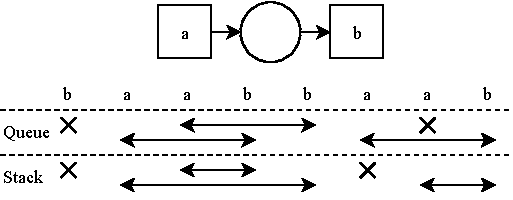
\includegraphics[scale=1]{figures/concept/overlap_strategy.pdf}
    \caption{A comparison of the queue and stack interaction extraction}
    \label{fig:stackqueue}
\end{figure}

Finally, the interaction sets for the local logs in Figure \ref{fig:mapstrats} of the running example are given in Figure \ref{fig:interactionstrats}. As mentioned before, $\func{sync\_strat}$ spreads out the incomplete interactions to all adjacent places while $\func{all\_strat}$ focuses it on the input places. Since swapped events can lead to two incomplete interactions, mapping log moves may lead to more incomplete interactions. In this example, using a stack or queue makes no difference.

\begin{figure}
    \centering
    \begin{tabular}{|l|c|c|}
    \hline
    \multirow{2}{*}{Local log} & \multicolumn{2}{|c|}{$\func{sync\_strat}$}  \\
     & $\CIS$ & $\IIS$ \\
    \hline
    $\Log_{p1}$ 
    & $\{ ((e_{11}^\tstart,t5),(e_{13}^a,t1)), ((e_{21}^\tstart,t5), (e_{22}^a,t1)) \}$ & $\{\}$ 
     \\
    $\Log_{p2}$ 
    & $\{ ((e_{13}^a,t1), (e_{14}^c,t3)), ((e_{22}^a,t1),(e_{\tau}^{t2},t2)) \}$ & $\{\}$ 
     \\
    $\Log_{p3}$ 
    & $\{ ((e_{\tau}^{t2},t2),(e_{23}^b, t4)) \}$ & $\{ ((e_{14}^c,t3),\missdown) \}$ 
     \\
    $\Log_{p4}$ 
    & $\{ ((e_{23}^b,t4),(e_{24}^\tend,t6)) \}$ & $\{ (\missup,(e_{15}^\tend,t6)) \}$
     \\
    \hline
    \hline
    \multirow{2}{*}{Local log} & \multicolumn{2}{|c|}{$\func{all\_strat}$} \\
    & $\CIS$ & $\IIS$ \\
    \hline
    $\Log_{p1}$ & $\{ ((e_{11}^\tstart,t5),(e_{13}^a,t1)), ((e_{21}^\tstart,t5), (e_{22}^a,t1)) \}$ & $\{\}$ \\
    $\Log_{p2}$ & $\{ ((e_{13}^a,t1), (e_{14}^c,t3)), ((e_{22}^a,t1),(e_{\tau}^{t2},t2)) \}$ & $\{\}$ \\
    $\Log_{p3}$ & $\{ ((e_{\tau}^{t2},t2),(e_{23}^b, t4)) \}$ & $\{ (\missup,(e_{23}^b,t4)), ((e_{14}^c, t3),\missdown) \}$ \\
    $\Log_{p4}$ & $\{ ((e_{12}^b,t4), (e_{15}^\tend,t6)), ((e_{23}^b,t4),(e_{24}^\tend,t6)) \}$ & $\{\}$ \\
    \hline
    \end{tabular}
    \caption{Continued running example with interaction sets}
    \label{fig:interactionstrats}
\end{figure}

\section{Time intervals} \label{timeintervals}
Until now, we extracted interactions of the log with places. This only uses the control-flow dimension and ordering of events. Since interactions also have the attributes $start$, $end$ and $duration$, it is possible to order them and spread them out over the time dimension. Complete interactions may also have a non-zero duration, so it is not trivial to filter them into time intervals. There are different types of overlap of an interaction with a time interval.
\begin{figure}
    \centering
    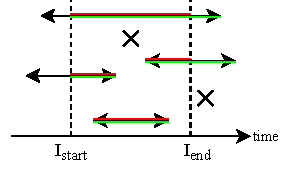
\includegraphics[scale=2]{figures/concept/timeinterval_overlap.pdf}
    \caption{Different types of overlap of interactions with a time interval}
    \label{fig:interactionoverlap}
\end{figure}
\begin{definition}[Time interval projections]
A time interval $[I_{start}, I_{end})$ has an inclusive start time $I_{start}$ and an exclusive end time $I_{end}$. The length of the interval is $L = I_{end} - I_{start}$.
The projections of an interaction set $\var{IS}$ ($\CIS$ or $\IIS$) to such a time interval are defined as functions with time interval parameters.
\begin{itemize}
    \item\emph{Touching}: $\mathit{T[I_{start}, I_{end})( IS ) = \set{int\in IS}{start(int) < I_{end} \wedge end(int)\ge I_{start}}}$
    \item\emph{StartingIn}: $\mathit{SI[I_{start}, I_{end})( IS ) = \set{int\in IS}{I_{start}\le start(int) < I_{end}}}$
    \item\emph{EndingIn}: $\mathit{EI[I_{start}, I_{end})( IS ) = \set{int\in IS}{I_{start}\le end(int) < I_{end}}}$
    \item\emph{ContainedIn}: $\mathit{CI[I_{start}, I_{end})( IS ) = \set{int\in IS}{I_{start}\le start(int) \le end(int) < I_{end}}}$
\end{itemize}
The actual overlap of a \emph{Touching} interaction $int \in \var{IS}$ with the time interval is between $\mathit{l\_limit = \max\{start(int), I_s\}}$ to $\mathit{r\_limit =  \min\{end(int), I_e\}}$, so $$\mathit{overlap[I_s,I_e)( int ) = \begin{cases} r\_limit - l\_limit & \text{if } start(int) < I_e \wedge end(int) \ge I_s  \\
0 & \text{otherwise}\end{cases}}$$
\end{definition}
Figure \ref{fig:interactionoverlap} shows some example interactions. The complete ones have arrowheads giving the $start$ and $end$ times and the incomplete ones are represented by \texttimes. All four complete ones are \emph{Touching}. The second one is also \emph{StartingIn}, the third one \emph{EndingIn} and the last one is both of those which makes it \emph{ContainedIn}. The top incomplete interaction is also everything while the bottom one is not touching at all. The overlap is colored red in the figure.

Finally, we define metrics for conformance, performance and process context.
For conformance, we propose two similar local fitness measures. One is based on the ratio of complete interactions and all interactions, while the other counts events instead of whole interactions. Since complete interactions are a pair of two events, the latter will always be higher, but it considers the actual time of occurrence more exactly.
\begin{definition}[Local fitness]
Let $\var{(CIS, IIS)}$ be a pair of sets of complete and incomplete interactions and $[I_s, I_e)$ be a time interval. The interactions starting in the interval are $\mathit{c\_start = SI[I_s, I_e)(\CIS)}$ and $\mathit{i\_start = SI[I_s, I_e)(IIS)}$ for complete and incomplete ones respectively.
$$\mathit{lfitness_{int}[I_s, I_e)( \CIS, \IIS ) = \begin{cases} \frac{|c\_start|}{|c\_start| + |i\_start|} & \text{if } |c\_start| + |i\_start| \neq 0\\
\text{undefined} & \text{otherwise}
\end{cases}}$$
The events from interactions inside the interval are $\var{ce\_start} = \set{e}{I_s \le time(e) < I_e \wedge e \in \set{e,e^\prime}{((e,t),(e^\prime,t^\prime))\in \CIS}}$ and $\var{ie\_start} = \set{e}{I_s \le time(e) < I_e \wedge ((e,t)) \in \IIS}$ for complete and incomplete interactions respectively.
$$\mathit{lfitness_{event}[I_s, I_e)( \CIS, \IIS ) = \begin{cases} \frac{|ce\_start|}{|ce\_start| + |ie\_start|} & \text{if } |ce\_start| + |ie\_start| \neq 0\\
\text{undefined} & \text{otherwise}
\end{cases}}$$
\end{definition}
If no interactions/events occur in the chosen time interval, the fitness is undefined. For the interval in Figure \ref{fig:interactionoverlap}, $\func{lfitness_{int}[I_{start}, I_{end})} = 0.67$ and $\func{lfitness_{event}[I_{start}, I_{end})} = 0.8$.

The current average sojourn time on a place is a measure for performance. The average is computed over complete interactions starting in the chosen interval. That means it is also undefined during intervals where no interactions occurred.
\begin{definition}[Local performance]
Let $\CIS$ be a set of complete interactions and $[I_s, I_e)$ be a time interval. Again, let $\mathit{c\_start = SI[I_s, I_e)(\CIS)}$.
$$\mathit{lperf[I_s,I_e)( \CIS ) = \begin{cases} \sum_{ci\in c\_start} duration(ci) / |c\_start| & \text{if } |c\_start|\neq 0\\
\text{undefined} & \text{otherwise} \end{cases}}$$
\end{definition}
$\func{lperf}$ describes how long (on average) cases that arrived at the place in the chosen interval eventually waited on there.

We propose three different metrics to try to measure the process context in terms of busyness at the current place during the chosen time interval. If many cases are currently waiting on this place, it will be busy.
\begin{definition}[Local busyness]
Let $\CIS$ be a set of complete interactions and $[I_s,I_e)$ be a time interval.
\begin{itemize}
    \item $\mathit{lbusyness_{c\_int}[I_s,I_e)( \CIS) = |SI[I_s,I_e)(CIS)|}$
    \item $\mathit{lbusyness_{activity}[I_s,I_e)( \CIS ) = \begin{cases} \sum_{ci \in CIS} overlap[I_s,I_e)(ci)/(I_e - I_s) & \text{if } I_s \neq I_e\\
    \text{undefined} & \text{otherwise} \end{cases}}$
    \item $\mathit{lbusyness_{remsojourn}[I_s,I_e)( \CIS ) = \sum_{ci\in T[I_s,I_e)(CIS)} (end(ci) - \max(start(ci),I_s))}$
\end{itemize}
\end{definition}

$\func{lbusyness_{c\_int}}$ is the number of complete interactions starting in the interval. Incomplete interactions may also inhibit performance since they are also in the log and actually occurred, so a variant $\func{lbusyness_{int}}$ counting all interactions may also be useful.
$\func{lbusyness_{activity}}$ is the sum of the ratios of overlap and the time interval size. The metric is relative to the interval size, so the interactions are weighed by their overlap which provides are more nuanced view on the busyness on a place during an interval. This is undefined for a time interval with the same start and end time.
$\func{lbusyness_{remsojourn}}$ is the total remaining sojourn time from the start of the interval of all touching interactions, shown in green in Figure \ref{fig:interactionoverlap}. In other words, if the place was a queue and could only handle one interaction after the other, it would take $\func{lbusyness_{remsojourn}}$ long to empty the queue. Instead of the total time, the average might also be interesting.

\section{Tying it all together} \label{alltogether}
The previous sections described the necessary process to arrive at metrics for conformance, performance and busyness. Given a system net $SN = (PN, M_i,M_f)$ and log $\Log$, the set of complete $\CIS$ and incomplete $\IIS$ interactions can be extracted for each individual place $p\in P$.
The metrics can then be calculated over time by dividing the whole process duration into a selected number of intervals or intervals of certain length like day, month or year. This yields a timeseries which can be used in statistical analysis to detect seasonality and trends.
By computing the relative standard deviation (standard deviation divided by mean) over the series or using other deviation metrics, one can also try to judge the stability of a certain metric over time. This way places can also be compared. Some might be in parts of the process that are quite streamlined and stable, while elsewhere the actual process execution may be more erratic in terms of conformance and performance. Figure \ref{fig:timeseriesschematic} shows a schematic of this on the running example model.
\begin{figure}
    \centering
    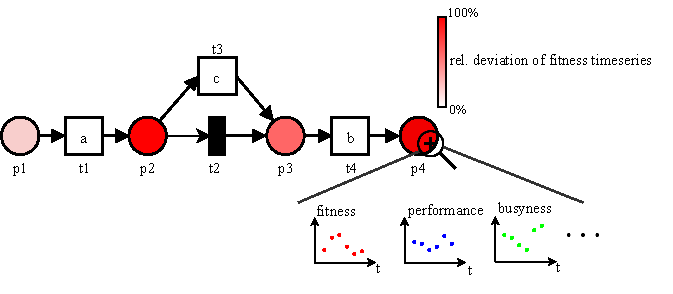
\includegraphics[width = \textwidth]{figures/concept/tyingtogether.pdf}
    \caption{Schematic result of applying the approach}
    \label{fig:timeseriesschematic}
\end{figure}
Another interesting application is finding correlations between these metrics. For example, does a high busyness value actually correlate with long sojourn times? In other words, how sensitive is this place to busyness? Or does a low conformance possibly lead to longer sojourn times? Since the $\CIS$ and $\IIS$ sets also contain the event and case data information, correlations can be extended to include those features. Which activity is often involved in incomplete interactions, and during which times? Do case attributes influence performance on this place? The localization of these questions to individual places and time frames makes it possible to find correlations which would be too weak to be detected over the whole log and process. For these purposes a dataset can be compiled containing all interactions with time and data information together with the metrics calculated for the duration of the interaction.

We also include another interesting aspect in our approach which is using the relative time since the case start. Every previously mentioned analysis can be performed for a relative time perspective by adjusting the intervals used for the metrics. It can be used to see after which time cases usually arrive at a place and if there are differences when they are later or earlier.

\chapter{Implementation} \label{chap:impl}
%%This chapter is used to show our implementation in ProM.  It can be split into 3 parts. 
%The first one is the Dfg method, including the weight update, process tree generation and petri net without long-term dependency generation.
% The second part is to add long-term dependency, it can be use as whole part or customized part into model, also removing the long-term dependency
% Evaluation part is the confusion matrix measurement.
%% Change implementation structure in this way::
%% 1. platform introduction, ProM + KNIME platforms
%% 2. No neccessary to describe the input right?? Aslo, there are another new concepts shown in the graph, which we need to avoid it. 
%% 3. then the screenshots to show the steps of the implementation
%% 4. If we introduce the property here, really, it will not help.. In this way, it can be fine.. But just add the introduction part for the KNIME
In this chapter, we begin with the introduction of implementation platforms for our methods and then show the use of those applications step by step.

\section{Implementation Platforms}
\subsection{Process Mining Platform -- ProM}
ProM is an open-source process mining tool in Java that is extensible by adding a set of plug-ins \cite{ProM}. ProM supports a wide variety of process mining techniques and is usually used for academic research. We implement the algorithm on ProM 6.8, which is the latest stable version. The corresponding plugin is \textbf{\emph{Repair Model By Kefang}} and released online \cite{MyPlugin}.

\subsection{KNIME}
KNIME Analytics Platform is an open-source software to help researchers analyze data. Multiple modules are integrated into this platform for loading, transforming and processing data. Researchers can achieve their goals by creating visual workflows composed of expected modules implemented as nodes with an intuitive, drag and drop style graphical interface, rather than focusing on any particular application area.

The reasons to integrate our techniques into KNIME are (1)KNIME is widely used in scientific research and benefits the application of our techniques;(2)KNIME supports automation of test workflow, which helps conduct more efficient experiments.  However, the integration requires additional development effort.
% here we need to change the name of our sections, because if we present them into a general way, so we need to show them in a general methods.
\section{Generate a Petri net}
Firstly two dialogs are poped up to set the arguments, such as the event classifier to  generate directly-follows graphs from event logs. Subsequently, a dialog is shown to set the Inductive Miner parameters. The parameters include the Inductive Miner variant and the noise threshold to filter the data. The dialog is displayed in Figure \ref{fig:dfg-IM-setting}.
\begin{figure}
	\centering
	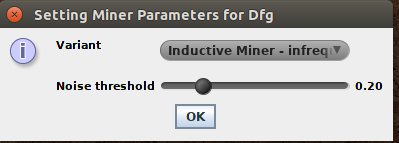
\includegraphics[scale=0.75]{figures/implementation/dfg-IM-setting.png}
	\caption{Inductive Miner Parameter Setting}
	\label{fig:dfg-IM-setting}
\end{figure} \\
After setting the parameters, process models  of process tree and Petri net without long-term dependency can be generated by Inductive Miner and displayed in the result view in Figure \ref{fig:dfg-IM-pn-without-lt}. 
\begin{figure}
	\centering
	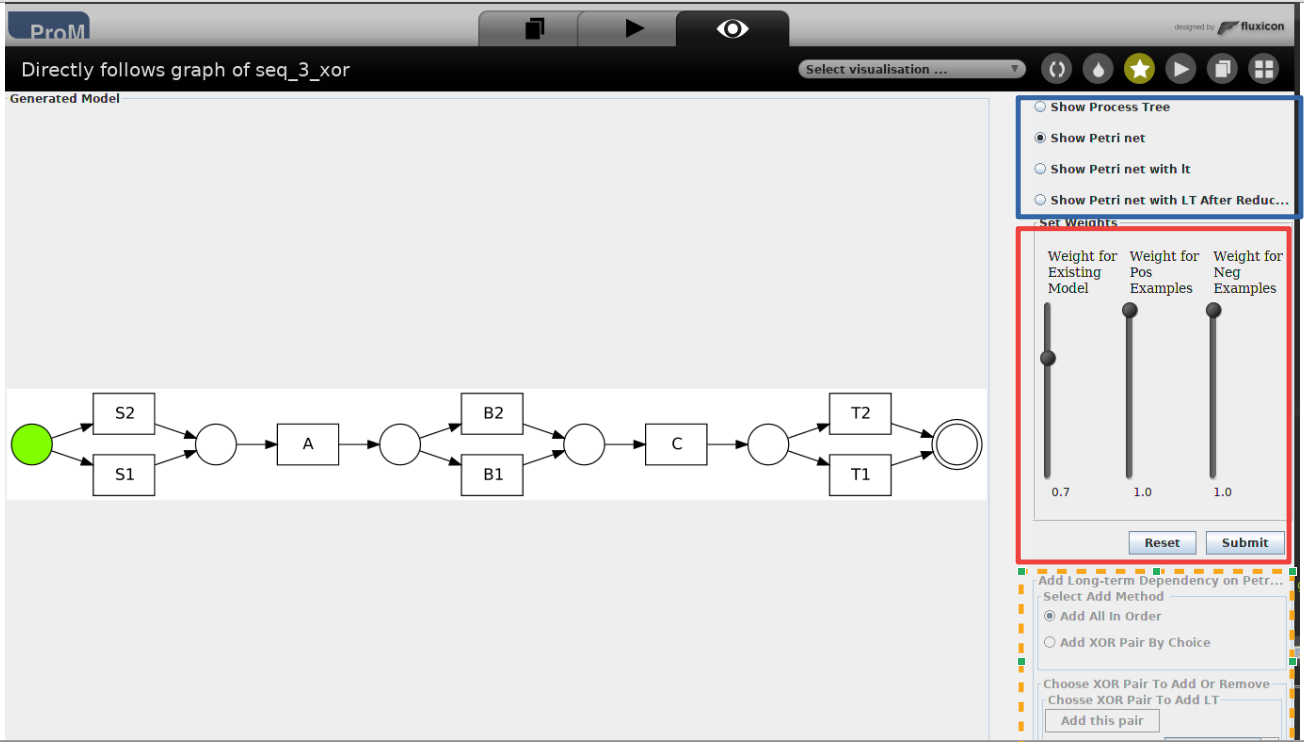
\includegraphics[width=\textwidth]{figures/implementation/dfg-IM-pn-without-lt.png}
	\caption{Generated Petri net without long-term dependency}
	\label{fig:dfg-IM-pn-without-lt}
\end{figure}
The left side is the model display area, where the right panel is to set the control parameters for the existing model, positive or negative instances. In interactive way, more flexibility is allowed by this plug-in to repair model. By default, the generated model type and the weight sliders are enabled at first. The control panel for adding long-term dependency are only triggered after choosing the option to repair model with long-term dependency. 

The model type is selected in the blue rectangle marked in Figure \ref{fig:dfg-IM-pn-without-lt}. It has 4 options to control the generated model type. Currently, the option "Show Petri net" is chosen, so the constructed model is Petri net without long-term dependency. The weights sliders are in red rectangle. They adjust the weights for the existing model, positive and negative instances. Once those options are submitted, different process models are mined under different weights. The rectangle in orange are the invisible part to control long-term dependency options. It will be discussed in the next section.

\section{Post Process to Add Long-term Dependency }
If we want to repair the Petri net with long-term dependency, one post procedure is triggered to add long-term dependency . This program in the background detects and puts places and silent transitions on Petri net directly mined from Inductive Miner to add long-term dependency. As comparison, the same weight setting is kept like the Figure \ref{fig:dfg-IM-pn-without-lt}, but the option to show a Petri net with long-term dependency is chosen. The resulted model is displayed in  Figure \ref{fig:dfg-IM-pn-with-lt}. 
\begin{figure}
	\centering
	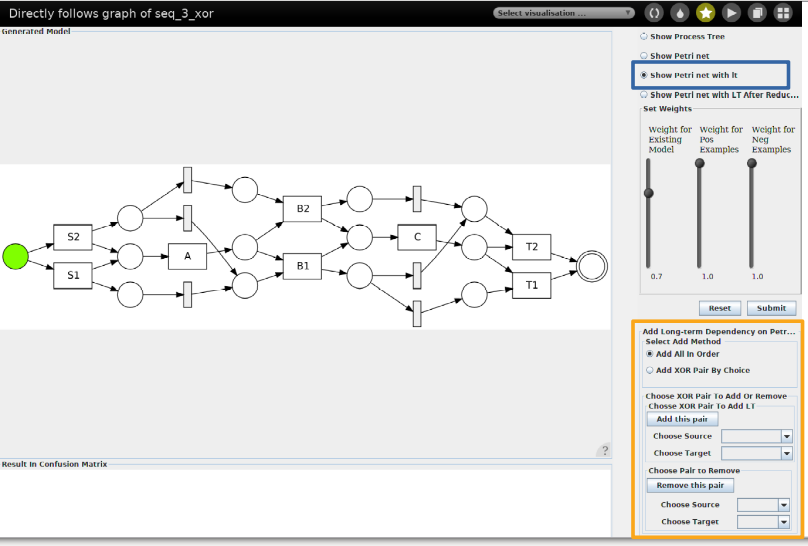
\includegraphics[width=\textwidth]{figures/implementation/dfg-IM-pn-with-lt.png}
	\caption{Petri Net with long-term dependency }
	\label{fig:dfg-IM-pn-with-lt}
\end{figure}

Meanwhile, the control part of adding long-term dependency turns visible in the orange rectangle like in Figure \ref{fig:dfg-IM-pn-with-lt}.  It has two main options, one is to consider all long-term dependencies existing in the model, the other is to choose the part manually. It allows more flexibility for users. Below those two options are the manual selection panels, including a control part to add and remove pair. As an example, the blocks Xor(S1,S2) and Xor(T1,T2) are chosen to add long-term dependency. It results in the model in Figure \ref{fig:dfg-IM-pn-with-lt-m}. 
\begin{figure}[h]
	\centering
	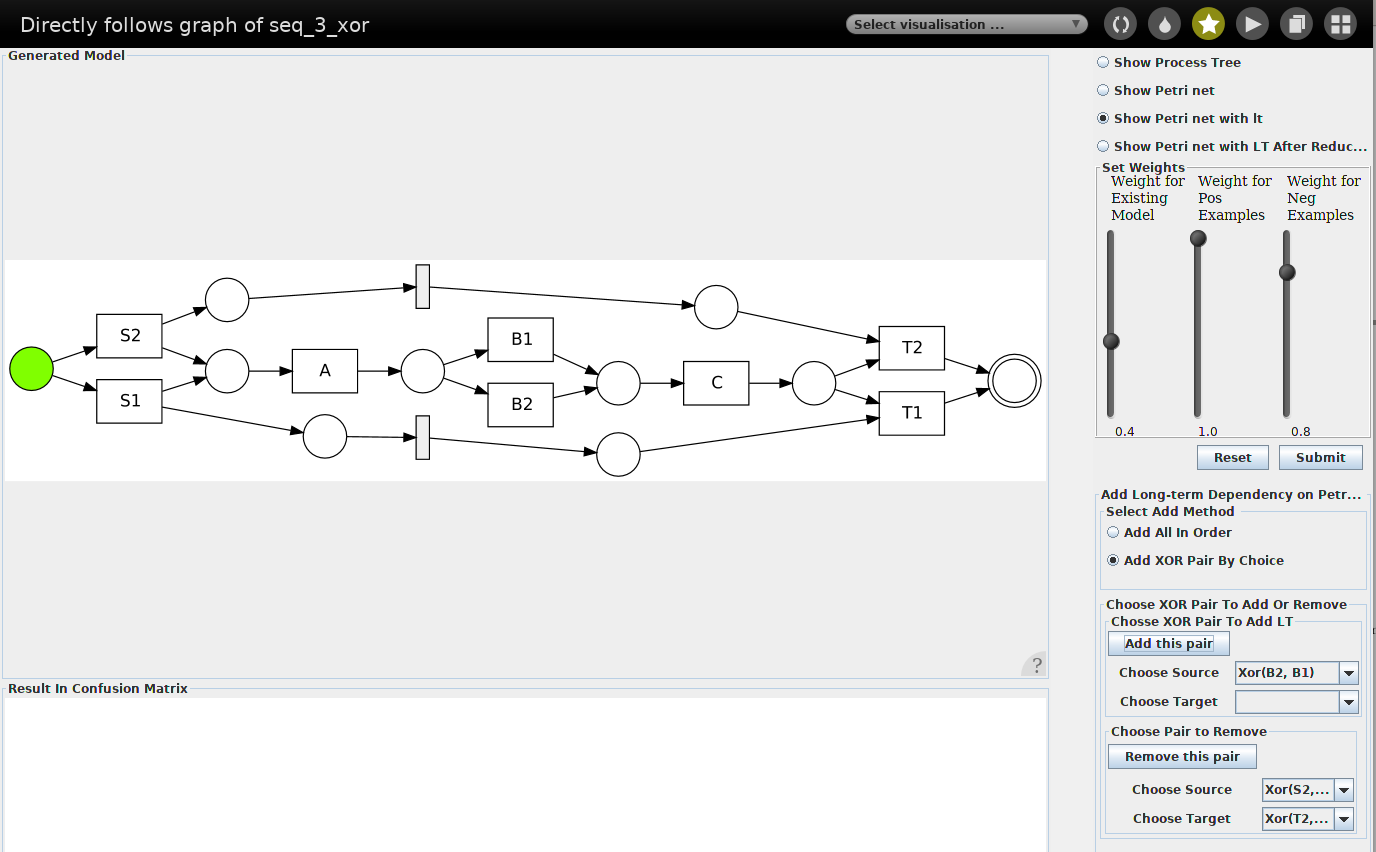
\includegraphics[width=\textwidth]{figures/implementation/dfg-IM-pn-with-lt-manual.png}
	\caption{Petri net with selected long-term dependency}
	\label{fig:dfg-IM-pn-with-lt-m}
\end{figure}
\section{Post Process to Reduce Redundant Silent Transitions and Places}
By choosing the option of \emph{Petri net with LT After Reducing} in model type, silent transitions and places are reduced to simplify the model.
Under the same setting in Figure \ref{fig:dfg-IM-pn-without-lt}, the simpler model in Figure \ref{fig:dfg-IM-pn-with-lt-r} is constructed, after the post processing of reducing silent transitions.
\begin{figure}[h]
	\centering
	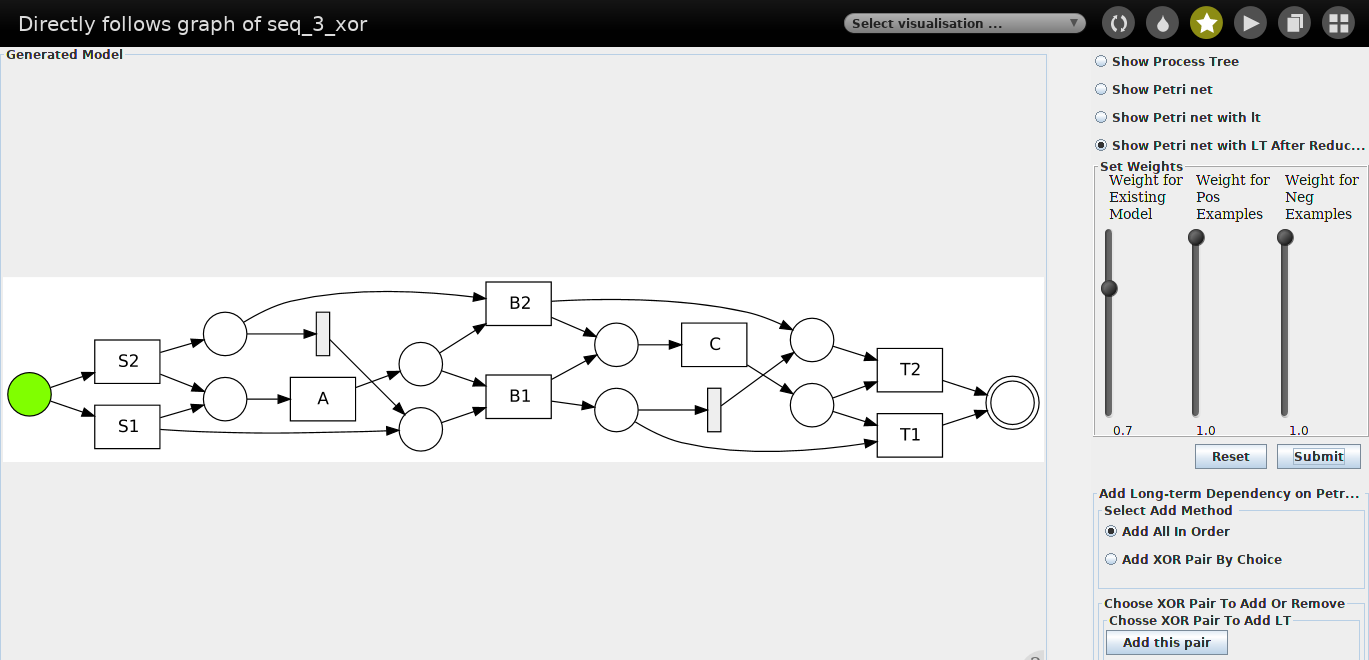
\includegraphics[width=\textwidth]{figures/implementation/dfg-IM-pn-with-lt-reduced.png}
	\caption{Petri net after reducing the silent transitions}
	\label{fig:dfg-IM-pn-with-lt-r}
\end{figure}

\section{Additional Feature to Show Evaluation Result}
Another feature in this plugin  is to show the evaluation result based on confusion matrix. With the brief evaluation result, it helps set the parameters for the optimal Petri net. 

After creating the current model in the left view, the evaluation program in background uses the event log and the current Petri net in the view as inputs. A naive fitness checking is applied on the repaired model with the event log. This procedure is based on the existing plugin in ProM -- \textbf{PNetReplayer}. This plugin checks if the trace fits the model and give out the one possible deviation with minimal cost. In our implementation, either the deviation on model or in trace is set with the same cost. Based on the deviation result and the label information on each trace, a confusion matrix is generated. Moreover, relative measurements like recall, precision are calculated and shown in the bottom of the left view in Figure \ref{fig:dfg-IM-cm}.  If the button of green rectangle in the right view \emph{Show Confusion Matrix} is pressed again, the program is triggered again and generates a new  confusion matrix result in the dark green dashed rectangle which will be listed above the previous result in light green dashes area. 
\begin{figure}
	\centering
	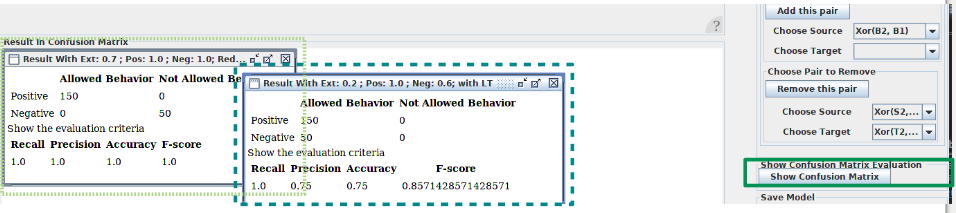
\includegraphics[width=\textwidth]{figures/implementation/dfg-IM-confusionmatrix.png}
	\caption{Generated Process Tree Model}
	\label{fig:dfg-IM-cm}
\end{figure}

\section{Integration into KNIME}
% this section describes the integration of our algorithm with KNIME, should we introduce some parts abotu them?? Yes, here about our real implementation, above should introduce the basic implementation steps.
\emph{Nodes} in the workflow represents different modules corresponding the plugins in ProM. Each node has certain input ports on the left side to represent the required parameters and  ports on the right to output result. By connecting the ports between nodes, data are passed and processed by one node after another. To integrate our algorithm into KNIME, other related modules on process mining are necessary, which can be divided into the following categories: 
% make a lot of work here to express your work
\begin{enumerate}
	\item Data importer and exporter. The importers and exporters for event logs, process trees and Petri nets are implemented to load and save basic data for Process Mining.
	\item Event logs manipulation. Nodes for splitting, sampling and assigning labels to event logs are implemented to benefit our experiments.
	\item Classic discovery algorithms. Inductive Miner and Alpha Miner are integrated into KNIME to provide baselines for our algorithm.
	\item Model enhancement. Our proposed method is integrated in KNIME to repair model in Petri net.
\end{enumerate}

To integrate our repair algorithm from ProM into KNIME, we need to create the workflow in the Figure \ref{fig:impl-KNIME}. After reading a Petri net by  \emph{PetrinetReader} and an event log by \emph{Import Event Log(XES)}, Node \emph{IncorporateNegInfo} applies the algorithm in this thesis to repair a model in Petri net with incorporating negative information. The outputs have different kinds of Petri nets to match the ones generated in ProM, eg. reduced Petri net with long-term dependency, Petri net without long-term dependency. In addition, we can evaluate our repaired model by using the node \emph{RepairEvaluator}. At last, we can save the repaired Petri net by \emph{PetrinetWriter}.
% give a screen shot and list the explaination on it.
\begin{figure}
	\centering
	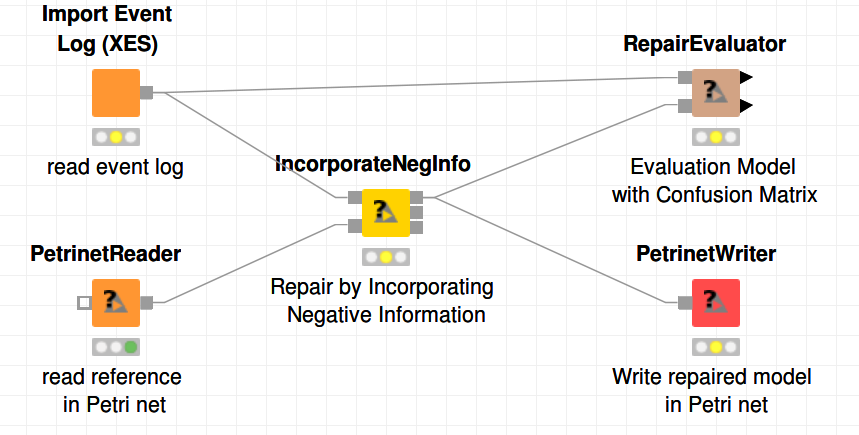
\includegraphics[width=\textwidth]{figures/implementation/implementation-KNIME.png}
	\caption{Integration of our repair techniques into KNIME}
	\label{fig:impl-KNIME}
\end{figure}


\chapter{Evaluation} \label{chap:eval}
%%This is the evaluation part, int includes the following parts.
% <1> Evaluation Metrics, explain the measurements chosen for this experiments
% <2> Test Platform in KNIME, introduced before so we don't really need to repeat it here
% Firstly, we validate our methods and make sure it works for the properties.. Then using the whole data to test the weights tend and also, if it handled the real life data. 
% <3.1> validation part to check the methods work for those situations, but not necessary;; Then big data test to show property to handle those situations. 
% <3> Test Cases Design, the parameters we want to compare, the cases
%   ==> synthetic data
%   ==> Real life data
%   ++ Data to test the property
This chapter presents an experimental evaluation of our repair techniques. At first, we define the evaluation criteria. Next, we briefly introduce the test platforms KNIME and relevant ProM plugins tools. Then, we conduct two kinds of tests. One is based one the demo example proposed in the introduction part, one is on the real life data. 
\section{Evaluation Measurements}
% First talk about our data and our model, then choose the confusion matrix as one measurements. But we should review the traditional measuremtns on process mining before introducing the confusion matrix. but we should also focus on the accuracy part and f-score.
We evaluate repair techniques based on the quality of repaired models with respect to the given event logs. In process mining, there are four quality dimensions generally used to compare the process models with event logs. 
\begin{itemize}
	\item \emph{fitness.} It quantifies the extent of a model to reproduce the traces recorded in an event log which is used to build the model. Alignment-based fitness computation aligns as many events from trace with the model execution as possible.  
	\item \emph{precision.} It assesses the extent how the discovered model limits the completely unrelated behavior that doesn't show in the event log. 
	\item \emph{generalization.} It addresses the over-fitting problem when a model strictly matches to only seen behavior but is unable to generalize the example behavior seen in the event log. 
	\item \emph{simplicity.} This dimension captures the model complexity. According to Occam's razor principle, the model should be as simple as possible.
\end{itemize}
% How to come to confusion matrix?? 
The four traditional quality criteria are proposed in semi-positive environment where only positive instances are available. Therefore, when it comes to the model performance, where negative instances are also possible, the measurement metrics should be adjusted. With labeled traces in the event log, the repaired model can be seen as a binary prediction model where the positive instances are supported while the negative ones are rejected. Consequently, the model evaluation becomes a classifier evaluation. 

% Describe its features and some derived measurements. 
Confusion matrix has a long history to evaluate the performance of a  classification model. A confusion matrix is a table with columns to describe the prediction model and rows for actual classification on data.  The repaired model can be seen a binary classifier and produces four outcomes- true positive, true negative, false positive and false negative shown in the Table \ref{tab:cm}.
\begin{itemize}
	\item True Positive(TP): The execution allowed by the process model has an positive performance outcome.
	\item True Negative(TN): The negative instance is also blocked by the process model.
	\item False Positive(FP): The execution allowed by the process model has an negative performance outcome.
	\item False Negative(FN):The negative instance is enabled by the process model.
\end{itemize} 
% confusion matrix
\begin{table}[]
	\caption{Confusion Matrix}
	\label{tab:cm}
	\begin{tabular}{ll|c|c|}
		\cline{3-4}
		&                   & \multicolumn{2}{c|}{repaired model}                                               \\ \cline{2-4} 
		\multicolumn{1}{l|}{}                                                                         &                   & \multicolumn{1}{l|}{allowed behavior} & \multicolumn{1}{l|}{not allowed behavior} \\ \hline
		\multicolumn{1}{|l|}{\multirow{2}{*}{\begin{tabular}[c]{@{}l@{}}actual \\ data\end{tabular}}} & positive instance & TP                                    & FN                                        \\ \cline{2-4} 
		\multicolumn{1}{|l|}{}                                                                        & negative instance & FP                                    & TN                                        \\ \hline
	\end{tabular}
\end{table}
Various measurements can be derived from confusion matrix. According to our model, we choose the following ones as the potential measurements. 
\begin{itemize}
	\item recall. It represents the true positive rate and is calculated as the number of correct positive predictions divided by the total number of positives.
	\[Recall = \frac{TP}{TP + FN}\]
	\item precision. It describes the ability of the repaired model to produce positive instances.
	\[Precision = \frac{TP}{TP + FP }\]
	%\item specificity. In opposite with recall, it measures the true negative rate.
	%\[Specificity = \frac{TN}{TN + FP}\]
	\item accuracy. It is the proportion of true result among the total number. It  measures in our case how well a model correctly allows the positive instances or disallows the negative instances.
	\[Accuracy = \frac{TP+TN}{TP+TN+FP+FN}\]
	\item F-score is is the harmonic mean of precision and recall.
	\[F_1 = \frac{2*Recall*Precision}{Precision + Recall}\]
\end{itemize}
Generally, there is a trade-off between the quality criteria. So the measurements are only used to compare specific aspects of our techniques.
\section{Experiment Platforms}
KNIME, as a scientific workflow analytic platform, supports automation of test workflow, which helps us repeat experiments efficiently. Yet, traditional evaluation plugins in ProM are not integrated into KNIME, so partial experiments are conducted in ProM.
\subsection{KNIME}
% this section describes how KNIME supports automatic test, FlowVariable and optimization parts of it.
KNIME supports automation of test workflow mainly through the following mechanisms. 
\begin{itemize}
	\item Loop Control Structure. KNIME provides a bunch of control nodes which support re-executing workflow parts.  Nodes representing \emph{Loop Start} appear in pairs with nodes for \emph{Loop Nodes}, the workflow between pairs is executed recursively in a fixed number, or until certain conditions are met. In our test, we repeat our repair techniques for different parameter settings by applying loop structure into KNIME workflow.
	\item Flow Variables. Flow Variables are used inside a KNIME workflow to parameter node settings dynamically. When it combines with loop control structure, tests with different settings is able to conduct automatically.
\end{itemize}
What's more, there are nodes provided by KNIME to optimize the value of some parameters with respect to a cost function. As long as a cost function is provides, KNIME is able to automatically optimize any kind of parameters. 
\subsection{ProM Evaluation Plugins}
%Here we discuss the plugins to test other aspects of our methods. 
Although KNIME offers a powerful approach to conduct experiments, the integration of traditional process mining evaluation plugins into KNIME is out of our capability due to the time limits. To evaluate repaired models with traditional metrics, we use an existing ProM plugin called \textbf{\emph{Multi-perspective Process Explorer}} \cite{mannhardt2015multi}. This plugin accepts  Petri net and an event log as inputs, and gives out fitness, and precision measurements which are based on the traditional alignment conformance checking. 
\section{Experiment Results}
\subsection{Test on Demo Example}
In this experiment, we aim to answer the question: Will our repair method overcome shortcomings of current techniques which are shown in the introduction chapter?  

% for situation 1, we can not get the ideal model, the reason is that we can not keep the model like just as it states, we can 

\subsection{Comparison To Other Techniques}
This section represents some situations where current repair techniques can't handle properly, while our algorithm gives out an improved repaired model. 

\emph{Situation 1}, unfit part!! added subprocess are too much!! Where the addition of subprocesses and loops are allowed, while the structure changes are impossible, 
Fahrland's method applies the extension strategy to repair model by adding subprocesses and loops in the procedure. It introduces unseen behavior into the model. However, if the behaviors which are already in the model is unlikely to be removed from the model. One simple example is shown in the following part. 

Dee's method is based on Fahrland's method. Deviations are calculated at first and used to build subprocesses for model repair. However, before building subprocesses, it classifies the deviations into positive and negative ones with consideration of trace performance. Only positive deviations are applied to repair model. Different to Fahrland's method, it improves the repaired model performance by limiting the introduced subprocesses. Still, it can't get rid of the defect mentioned before. 

\emph{Situation 2}, For fitted data in the model, can not recognize them!! where overlapped data noise can not be recognized, trace variant with more negative effect is treated as positive and kept in the model, which we should delete them.   
% Here we want to give an example of the overlapped data, compared to IM rediscoverty, easy.. But for Dees' method, firstly, they have labeled data; The analyzed the deviations of them, but when one deviation dominates, then the tree can not see the others. Some data are ignored..

\emph{Situation 3}, with long-term dependency!! fitted part or new added part!! none of the current techniques can handle this problem yet.
Simple examples listed, but will this repeat the last section?? 


% Conclusion part
For one exclusive choices, 
but with long-term dependency detected and added in the model, precision and accuracy increase, since model with long-term dependency blocks the negative information by adding transitions and places to limit activity selection. 

\subsection{Test On Real life Data}
% here we will list all the data here but before describe the test data
\subsubsection{Data Description}
\subsubsection{Test Result}
% we don't need to transfer page to landscape view, because we have many rows too.
	\begin{table}[]
		\centering
		\caption{Test Result on BPI15-M1 data}
		\resizebox{\textwidth}{!}{
		\begin{tabular}{lll|llllllll|ll}
			\hline
			\multirow{2}{*}{\thead{event \\ log}} & \multirow{2}{*}{\thead{reference \\ model} }                &    \multirow{2}{*}{\thead{method}}       & \multicolumn{8}{l}{ \thead{confusion matrix metrics}}                              & \multicolumn{2}{|l}{\thead{traditional metrics}} \\
			\cline{4-13}
			 &  &     &
			  \thead{TP}  & \thead{FP} & \thead{TN}  & \thead{FN}  & \thead{recall} & \thead{precision} & \thead{accuracy} & \thead{F1}   & \thead{fitness}           & \thead{precision}           \\
			  \hline
			D1.1      & M1              & IM & 137 & 48 & 118 & 289 & 0.32   & 0.74      & 0.43     & 0.45 & ?                 & ?                   \\
			D1.1      & M1              & Fahland   & 0   & 0  &     &     &        &           &          &      &                   &                     \\
			D1.3      & M1              & Dees      &     &    &     &     &        &           &          &      &                   &                     \\
			D1.3      & M1              & dfg       &     &    &     &     &        &           &          &      &                   &                     \\
			D1.1      & M2              & IM  &     &    &     &     &        &           &          &      &                   &                     \\
			D1.1      & M2              & Fahland   &     &    &     &     &        &           &          &      &                   &                     \\
			D1.3      & M2              & Dees      &     &    &     &     &        &           &          &      &                   &                     \\
			D1.3      & M2              & dfg       &     &    &     &     &        &           &          &      &                   &                     \\
			D1.1      & M3              & IM  &     &    &     &     &        &           &          &      &                   &                     \\
			D1.1      & M3              & Fahland   &     &    &     &     &        &           &          &      &                   &                     \\
			D1.3      & M3              & Dees      &     &    &     &     &        &           &          &      &                   &                     \\
			D1.3      & M3              & dfg       &     &    &     &     &        &           &          &      &                   &                     \\
			D1.1      & M4              & IM  &     &    &     &     &        &           &          &      &                   &                     \\
			D1.1      & M4              & Fahland   &     &    &     &     &        &           &          &      &                   &                     \\
			D1.3      & M4              & Dees      &     &    &     &     &        &           &          &      &                   &                     \\
			D1.3      & M4              & dfg       &     &    &     &     &        &           &          &      &                   &                     \\
			D2.1      & M1              & IM &     &    &     &     &        &           &          &      &                   &                     \\
			D2.1      & M1              & Fahland   &     &    &     &     &        &           &          &      &                   &                     \\
			D2.3      & M1              & Dees      &     &    &     &     &        &           &          &      &                   &                     \\
			D2.3      & M1              & dfg       &     &    &     &     &        &           &          &      &                   &                     \\
			D2.1      & M2              & IM  &     &    &     &     &        &           &          &      &                   &                     \\
			D2.1      & M2              & Fahland   &     &    &     &     &        &           &          &      &                   &                     \\
			D2.3      & M2              & Dees      &     &    &     &     &        &           &          &      &                   &                     \\
			D2.3      & M2              & dfg       &     &    &     &     &        &           &          &      &                   &                    
		\end{tabular}}
	
	\end{table}


\chapter{Related Work} \label{chap:related}
\input{chapters/"related work.tex"}

\chapter{Conclusion} \label{chap:conclusion}
% what kind of conclusion do you want to get?? My method works in some cases while other methods can not. 
% <1> deal with some situations
% <2> improve precision and accuracy compared to existing model
% Further work:<1> consider multiple KPIs in the model and adjust them
%    <2> Add long-term dependency directly on Petri net
%    <3> deal with the unsound model and fix them in some way
%    <4> simply using the threshold to generate model, but want to integrate with machine learning and generate good model

% Also, some limitations about our methods, we need to point them out.
%% can not give out the best setting
%% it is absoulte values, not vary due to the problem.

%%% add ``References'' section to TOC
%\phantomsection

\bibliography{bibl} \addcontentsline{toc}{chapter}{Bibliography}

\end{document}